\documentclass[11pt, a4paper, german]{article}
\usepackage{mathptmx}
\usepackage{booktabs}
\usepackage{algorithmic}
\usepackage[titlenotnumbered, vlined, ruled]{algorithm2e}
\usepackage{amsfonts}
\usepackage{amsmath}
\usepackage{amssymb}
\usepackage{amsthm}
\usepackage{mathtools}

\usepackage{array}
\usepackage[ngerman]{babel}
\usepackage[utf8]{inputenc}
\usepackage{color}
\usepackage{enumerate}
\usepackage{graphicx}
\usepackage{hyperref}
\usepackage{latexsym}
\usepackage{pdflscape}
\usepackage{makecell}
\usepackage{makeidx}
\usepackage{multirow}
\usepackage{pdfpages}
\usepackage{tikz}
\usepackage{tkz-fct}
\usepackage{tkz-graph}
\usetikzlibrary{patterns}
\usepackage{upgreek}
\usepackage{standalone}
\usepackage{slantsc}
\usepackage{lmodern}
\usepackage[labelformat=empty, font={scriptsize}]{subcaption}
\usepackage[labelformat=empty, font={scriptsize}]{caption}
\usepackage{pgfplots}
\usepackage{pgfplotstable}
\usepackage{circuitikz}
\usepackage{changepage}

\usetikzlibrary{shapes}
\usetikzlibrary{matrix, arrows,fit,shapes.gates.logic.US,shapes.gates.logic.IEC,calc,backgrounds,decorations.pathmorphing}




\DeclarePairedDelimiter\abs{\lvert}{\rvert}
\makeatletter
\let\oldabs\abs
\def\abs{\@ifstar{\oldabs}{\oldabs*}}
%
\let\oldnorm\norm
\def\norm{\@ifstar{\oldnorm}{\oldnorm*}}
\makeatother

\newcommand{\area}{\text{area}}
\newcommand{\uniquecone}{\text{unique\_cone}}
\newcommand{\uniquearea}{\text{unique\_area}}

\pgfplotsset{compat=1.8}

%
% Colors
%
\definecolor{darkblue}{RGB}{10, 0, 128}
\definecolor{grey}{RGB}{128, 128, 128}
\definecolor{darkred}{RGB}{180, 0, 0}
\definecolor{darkgreen}{RGB}{0, 100, 0}
\definecolor{lightgrey}{RGB}{210,210,210}
\newcommand{\RED}[1]{\textcolor{darkred}{#1}}
\newcommand{\BLUE}[1]{\textcolor{darkblue}{#1}}
\newcommand{\GREEN}[1]{\textcolor{darkgreen}{#1}}
\renewcommand{\emph}[1]{{\BLUE{#1}}}

\definecolor{darkRed}{rgb}{0.6,0,0}
\definecolor{lightRed}{rgb}{1,0.75,0.75}
\definecolor{darkGreen}{rgb}{0,0.5,0}
\definecolor{PineGreen}{rgb}{0.01,0.5,0.45}
\definecolor{darkBlue}{rgb}{0, 0, 0.75}
\definecolor{CornflowerBlue}{rgb}{0.15,0,0.7}
\definecolor{lightBlue}{rgb}{0.75,0.75,1}
\definecolor{grey}{rgb}{0.5,0.5,0.5}
\definecolor{black}{rgb}{0,0,0}
\definecolor{red}{rgb}{1,0,0}
\definecolor{green}{rgb}{0, 0.8, 0.3}
\definecolor{blue}{RGB}{10, 0, 128}
\definecolor{yellow}{rgb}{1,1,0}
\definecolor{orange}{rgb}{1,0.6,0}
\definecolor{cyan}{rgb}{0,0.7,1}
\definecolor{purple}{rgb}{0.5,0,0.8}

\newcommand\mycommfont[1]{\footnotesize\ttfamily\textcolor{darkGreen}{#1}}{}{}
\SetCommentSty{mycommfont}
\SetArgSty{textup}
\renewcommand\thempfootnote{\arabic{mpfootnote}}
\renewcommand{\thealgocf}{}

% \SetKwComment{Comment}{}{}

%
% Shorthands
%
\newcommand{\BL}{\textsc{BonnLogic}}
\newcommand{\Restr}{\textsc{And-Or}-Path Restructuring}
\newcommand{\AOP}{\textsc{And-Or}-Path}
\newcommand{\aop}{\textsc{And-Or}-path}

% \pgfpagesuselayout{resize to}[a4paper,landscape,border shrink=5mm]

% CONFIGURE PACKAGES

% NEW COMMANDS

\newcommand{\bl}[1]{\index{BonnLogic@\textsc{BonnLogic}!#1}}

\newcommand{\brent}[1]{\index{Brents adder@Brent's adder!#1}}

\newcommand{\ceil}[1]{\left\lceil #1 \right\rceil}

\newcommand{\delay}{\mathrm{delay}}

\newcommand{\depth}{\mathrm{depth}}

\newcommand{\floor}[1]{\left\lfloor #1 \right\rfloor}

\newcommand{\ld}{\log_{2}}

\newcommand{\loq}{\log_{\phi}}

\newcommand{\mini}[4]{\begin{minipage}{#1\linewidth}#3\end{minipage}\hfill\begin{minipage}{#2\linewidth}#4\end{minipage}}

\newcommand{\minialt}[4]{\centering{\begin{minipage}{#1\linewidth}#3\end{minipage}\begin{minipage}{#2\linewidth}#4\end{minipage}}}

\newcommand{\myindex}[1]{\emph{#1}\index{#1}}

\newcommand{\npfx}[1]{\index{non-prefix adders!#1}}

\newcommand{\OPT}{\mathrm{OPT}}

\newcommand{\pfx}[1]{\index{parallel prefix graph!#1}}

\newcommand{\size}{\mathrm{size}}

\newcommand{\sset}[1]{\left\{#1\right\}}

\newcommand{\todo}[1]{
  %\textcolor{red}{(TODO: \emph{#1})}
}

\newcommand{\vare}{\varepsilon}


% IMAGES

\newcommand{\tikzs}[2]{
  \centering
  \includegraphics[width=#1\linewidth]{images/#2.pdf} %fast
  %\ttikz{#2.tex}{#1} %slow
}
\newcommand{\tikzc}[3]{
  \centering{
    \includegraphics[width=#2\linewidth]{images/#3.pdf}
    \caption{#1}
    \label{fig:#3}%
  }
}
\newcommand{\tikzcc}[3]{
  \centering{
    \resizebox{#2\linewidth}{!}{
      \begin{tikzpicture}
        \input{images/#3}
      \end{tikzpicture}
    }
    \caption{#1}
    \label{fig:#3}%
  }
}
\newcommand{\ntikz}[1]{
  \begin{tikzpicture}
    \input{images/#1}
  \end{tikzpicture}
}
\newcommand{\ttikz}[2]{
  \centering{
    \resizebox{#2\linewidth}{!}{
      \begin{tikzpicture}
        \input{images/#1}
      \end{tikzpicture}
    }
  }
}
\newcommand{\ttikzfig}[3]{
  \begin{figure}[hbt]
    \centering{
      \resizebox{#2\linewidth}{!}{%
        \begin{tikzpicture}
          \input{images/#3}
        \end{tikzpicture}%
      }%
    }%
    \caption{#1}
  \end{figure}
}
\newcommand{\tikzfigs}[3]{
  \begin{figure}[hbt]%
    \centering{%
      \includegraphics[width=#2\linewidth]{images/#3.pdf}
      \caption{#1}%
      \label{fig:#3}%
    }%
  \end{figure}%
}
\newcommand{\tikzfigsc}[3]{
  \begin{figure}[hbt]%
    \centering{%
      \resizebox{#2\linewidth}{!}{%
        \begin{tikzpicture}
          \input{images/#3}
        \end{tikzpicture}%
      }%
      \caption{#1}%
      \label{fig:#3}%
    }%
  \end{figure}%
}
\newcommand{\tikzfig}[2]{
  \tikzfigs{#1}{1}{#2}
}


\usepackage{standalone}
\usepackage{slantsc}
\usepackage{lmodern}
%\newcounter{algorithm}
%\newtheorem{algorithm}[algorithm]{Algorithm}

\theoremstyle{plain}
\newtheorem{theorem}{Theorem}[section]
\newtheorem{cor}[theorem]{Corollary}
\newtheorem{lemma}[theorem]{Lemma}
\newtheorem{conj}[theorem]{Conjecture}
\theoremstyle{definition}
\newtheorem{definition}[theorem]{Definition}
\theoremstyle{remark}


\usepackage{caption}
\usepackage{subcaption}
\clubpenalty = 10000
\widowpenalty = 10000 
\displaywidowpenalty = 10000
\usepackage{Titelseite}
\usepackage{natbib}
\usepackage{bbold, verbatim}
\usepackage{graphicx}
\newcommand{\TM}{Technology  Mapping }
\DeclareMathOperator*{\argmin}{arg\,min}

%Namen des Verfassers der Arbeit
\author{Alexander Zorn}
%Geburtsdatum des Verfassers
\geburtsdatum{26. Mai 1996}
%Gebortsort des Verfassers
\geburtsort{Bonn}
%Datum der Abgabe der Arbeit
\date{\today}

%Name des Betreuers
% z.B.: Prof. Dr. Peter Koepke
\betreuer{Betreuer: Prof. Dr. Stephan Held}
%Name des Instituts an dem der Betreuer der Arbeit tätig ist.
\zweitgutachter{Zweitgutachter: 
Prof. Dr. Dr. h.c. Bernhard Korte}
%z.B.: Mathematisches Institut
\institut{Forschungsinstitut f\"ur Diskrete Mathematik}
%Titel der Bachelorarbeit
\title{Algorithmen f\"ur das \TM}
%Do not change!
\ausarbeitungstyp{Bachelorarbeit Mathematik}



\begin{document}
%\raggedright

\setlength{\parindent}{0pt} %kein Einrücken zu Beginn eines Absatzes
%Beweis:
\renewcommand{\proofname}{Beweis:}
\maketitle

\setcounter{tocdepth}{2}
\tableofcontents
\newpage 
\section{Einleitung}
\label{sec:einleitung}
Die ständig komplexer werdenden Anforderungen an die Informationstechnologie verlangen nach immer leistungsfähigeren Computerchips. \\
Die sich hieraus ergebenden Anforderungen an die Chipentwicklung wurden bereits 1965 von Gordon Moore in "Moore's law"  \cite{Moore} beschrieben; hiernach ist regelmäßig eine Verdopplung der Integrationsdichte, der Anzahl von Transistoren pro Flächeneinheit erforderlich und auch bisher technisch realisierbar. Nach \cite{Khan} wird dies jedoch in absehbarer Zeit nicht mehr möglich sein, wodurch Lösungsansätze durch Diskrete Mathematik, die auch Thema dieser Arbeit sind, einen wichtigen Beitrag für das Chip-Design leisten. \\
Derzeit beträgt die Dichte an Transistoren, die zu einem integrierten Schaltkreis auf einem Chip miteinander verbunden sind, bis zu mehrere Milliarden. Diese sind so angeordnet, dass sie gemeinsam eine vorgegebene logische Funktion errechnen können. Die Aufgabe des Chip-Designs ist es, einen herstellbaren Chip zu entwerfen, der eine vorgegebene logische Funktion realisiert.\\

\begin{wrapfigure}{r}{6.2cm}
	\scalebox{1}[-1]{
		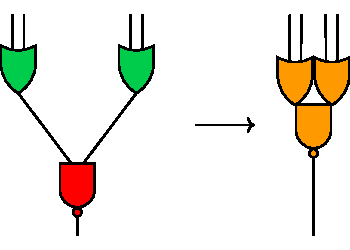
\includegraphics[]{pictures/compiled/einfBsp}
	}
		\caption{Zwei Realisierungen der logischen Funktion $\neg((w\lor x) \land (y \lor z))$}
		\label{bild:einfbsp}
\end{wrapfigure}
Mithilfe von aus wenigen Transistoren konstruierten Bauteilen (genannt Gates, z.B.: AND, OR, INV, OAI ...), lässt sich eine logische Funktion nachbilden. Abbildung \ref{bild:einfbsp} (linker Teil) zeigt dies an einem kleinen Beispiel.  Die Realisierung einer solchen Funktion ist jedoch nicht eindeutig wie Abbildung \ref{bild:einfbsp}  zeigt. 
Die Größe der Menge aller möglichen Baupläne (später Circuits) für eine logische Funktion hängt maßgeblich von den auf dem Chip zur Verfügung stehenden Bauteilen sowie von dem Aufbau der Funktion, ab. Hierdurch bedingt ergeben sich eine Vielzahl von  Möglichkeiten eine logische Funktion zu realisieren.\\
 Jedes Bauteil hat entsprechend spezifische physikalische Eigenschaften an Größe, Geschwindigkeit (Delay) etc.. Demnach hat auch jeder Circuit entsprechende Eigenschaften. \\
Ziel des Technology Mappings ist es für eine gegebene logische Funktion eine Realisierung zu finden, welche eine Kostenfunktion, bestehend aus den physikalischen Eigenschaften, optimiert. Die Wahl der Lösung hat direkte Auswirkungen auf die  Schnelligkeit, die Größe und den Stromverbrauch des fertigen Chips. Hierbei geht das \TM von einer bereits realisierten logischen Funktion aus und baut diese zu einer möglichst kostengünstigen Variante um. \\
Der optimale mögliche Umbau lässt sich bei kleinen oder eingeschränkten gegebenen Bauplänen noch in kurzer Zeit finden. Die Lösung dieses Problems für allgemeine Baupläne und Kostenfunktionen ist jedoch ein NP-vollständiges Problem. Aus diesem Grund entwickelt die vorliegende Arbeit eine Heuristik, welche für sehr große Baupläne, bestehend aus mehreren 10.000 Bauteilen, in möglichst kurzer Zeit einen kostenoptimierten Umbau approximiert.\\

Aufbauend auf den Arbeiten von Keutzer \cite{DAGON} und  Elbert \cite{Elbert} wird ausgehend von einem Kern-Algorithmus auf eingeschränkten Instanzen in Kapitel \ref{sec:terminologie&grundl} ein polynomielles Approximationsschema für einen beliebigen Approximationsfaktor $\epsilon > 0$ und daraus eine Heuristik in Kapitel \ref{sec:allg_algorithmus} entwickelt. Anschließend wird diese Heuristik  in Kapitel \ref{sec:erw_der_heuristik} an möglichst allgemeine Instanzen und weitere reale Gegenbenheiten angepasst. Mithilfe des Resource Sharing Algorithmus wird in Kapitel \ref{sec:resource_sh} die entwickelte Heuristik Teil einer allgemeinen Logik-Optimierung von Circuits. Abschließend wird in Kapitel \ref{sec:analyse} die Implementierung der vorgestellten Heuristik ausführlich analysiert.

\section{Terminologie und Kern-Algorithmus}
\label{sec:terminologie&grundl}
\subsection{Grundlegende Definitionen}
\label{subsec:grundlegende_definitionen}
Es folgen einige grundlegende Definitionen, die für die Beschreibung des Problems erforderlich sind.

\begin{definition}{Boolesche Variable und Funktion: } \\
Eine boolesche Variable ist eine Variable mit Werten in $ \{ 0 , 1 \} $.
Sei $ n, m \in \mathbb{N}$. Eine boolesche Funktion ist eine Funktion $ f : \{ 0 , 1 \}^n \rightarrow \{ 0 , 1 \}^m $ mit $n$ Inputs und $m$ Outputs. 
\end{definition}

\begin{definition}{Gate und Library:}\label{def:gate}\\
Ein Gate $g$ mit Eingangsgrad (arity) $ n \in \mathbb{N}$ ist ein Tripel $(f_g, d_g, area_g)$. Hierbei sind $d_g, area_g \in \mathbb{R}_{\geq 0}$. Des Weiteren ist $f_g$ eine boolesche Funktion mit $ f_g : \{0,1\}^n \rightarrow \{0, 1\} $. \\
Eine Library L ist eine Menge von Gates und sei \\ 
$fanin_{max} := max\{ arity(g) | g \in L \}$.
\end{definition}
\begin{figure}[h]
\begin{center}
 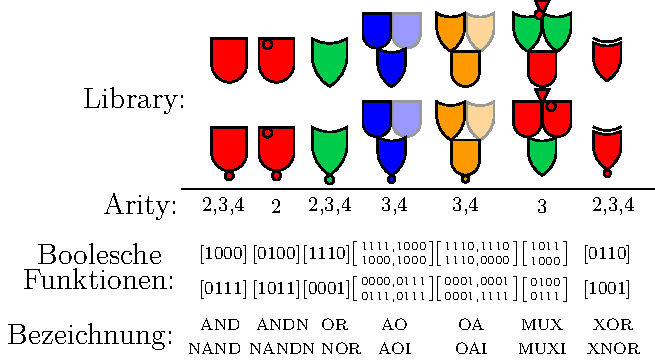
\includegraphics[height = 200pt]{./pictures/compiled/new_library.pdf}
 \caption{Beispiel einer Library}
 \label{bild:new_library}
\end{center}
\end{figure}
In der Praxis treten Gates mit gleicher Funktionalit\"at sehr h\"aufig auf. Die unterscheiden sich hinsichtlich Gr\"o{\ss}e, Geschwindigkeit und Stromverbrauch etc.. Die Entscheidung welche Variante des Gates implementiert wird, wird mit einem Gate-Sizing Algorithmus getroffen. Eine ausf\"uhrliche Beschreibung und effiziente L\"osung dieses Problems findet sich in \cite{GateSizing}. In dieser Arbeit wird davon ausgegangen, dass in einer Library keine logische Funktion durch zwei verschiedene Elemente realisiert wird.\\
Abbildung \ref{bild:new_library} gibt einen Überblick über eine praktisch genutzte Library. Jedes dieser Gates liegt in diesem Beispiel auch in einer invertierten Version vor (zweite Reihe der Library). Des Weiteren ist es für gewöhnlich der Fall, dass von einem Gatetyp mehrere Varianten bezüglich der Anzahl seiner Inputs vorhanden sind. Die Zeile mit dem Titel Arity gibt einen Überblick darüber, welche Variationen auf Chips üblich sind.\\
Wie gerade definiert, realisiert jedes Gate eine boolesche Funktion. In der entsprechenden Zeile der Abbildung ist für jedes Gate (einmal nicht invertiert und einmal invertiert) die  Funktion, für 2, 3 oder 4 Inputs, abgebildet. Dies geschieht in folgendem Format: Der Ausdruck $[1,...,2^{arity(g)} ]$ gibt für ein Gate $g$ an der Stelle $i \in \{1,...,2^{arity(g)}\}$ die Wahrheitsbelegung des Outputs bei Inputbelegung $i_2$ ($i$ dargestellt in Binärschreibweise) an. Es ist üblich an den Namen eines Gates die Arity zu knüpfen. Beispiel: AND2. \\

Die $area_g$ gibt die Größe des physikalischen Bauteils an und $d_g$ beschreibt die Zeit, die ein Signal braucht, um von den Inputs des Gates zu seinem Output zu gelangen. Dieser Wert lässt sich noch weiter differenzieren, indem man $d_g \in \mathbb{R}^{arity(g)}$ wählt und somit Zeiten für jeden der Inputs angegeben werden können. Hierauf wird jedoch erst in Kapitel \ref{sec:weitere_opt_krit} eingegangen. \\
Wenn die Signale der Inputs nicht zur selben Zeit ankommen, wird, falls nichts anderes angegeben, gewartet, bis das letzte Signal das Gate erreicht.

\begin{definition}{Circuit:}\\
Ein Circuit ist ein gerichteter kreisfreier Graph (directed acyclic graph DAG) mit der Eigenschaft: Jeder Knoten gehört zu einer der aufgelisteten Kategorien: 
\begin{itemize}
\item {\bf Inputs }mit Eingangsgrad Null.
\item{\bf Gates} mit mindestens einer eingehenden und mindestens einer ausgehenden Kante.
Diese Knoten entsprechen den Gates (Definition \ref{def:gate}) und darüber hinaus gilt: An jeder eingehenden Kante kann ein Inverter liegen.
\item{\bf Outputs} mit genau einer eingehenden und keiner ausgehenden Kante.
\end{itemize}
Ein Gate mit mehr als einer ausgehenden Kante wird auch Multifanoutgate genannt.\\
Ein Circuit realisiert durch Verschachtelung der booleschen Funktionen seiner Gates ebenfalls eine boolesche Funktion. \\
Zwei Circuits heißen äquivalent, wenn sie die gleiche boolesche Funktion realisieren.
\end{definition}

In den Abbildungen dieser Arbeit werden die Outputs eines Circuits nicht mit angegeben da eindeutig ist, welches Gate Vorgänger eines Outputs ist. Diese Knoten sind gemeint wenn von den Outputs des Graphen gesprochen wird. 

Es is möglich, dass das Signal eines Gates sowohl direkt in einen Output-Knoten geleitet wird als auch noch weiter verarbeitet wird. Weitere Informationen über den Umgang mit mehreren Outputs befinden sich in Kapitel \ref{sec:outputs}.\\
In einem Circuit lassen sich Teilgraphen durch ein Gate der Library austauschen. Voraussetzung für einen solchen Tausch ist, dass der veränderte Circuit äquivalent zu dem Original ist. Dies wird in den folgenden Definitionen formalisiert. 

\begin{definition}{Match und Kandidat:}\\
Sei $g$ ein Gate in einem Circuit $C$. Ein (invertiertes) Match $m$ auf $g$ ist ein Tupel $(p_m, X_m, f_m, inv_m)$ welches Folgendes enthält:
\begin{itemize}
\item Ein Gate $p_m$ der Library
\item Eine Menge $X_m$ von Knoten aus dem Circuit und eine Bijektion $ f: X_m \rightarrow inputs(p_m)$
\item Eine Funktion $ inv_m : inputs(p_m) \rightarrow \{not\_inv , inv \}$
\end{itemize}
sodass der Circuit $C'$, welcher durch den Austausch des Subcircuits von $X_m$ bis $g$ durch das Match (mit den durch $inv_m$ definierten Invertern an den Inputs) entsteht, äquivalent zu C ist.
Ein invertiertes Match auf $g$ ist ein Match auf $g$ mit einem Inverter an jedem seiner Outputs.\\
Ein Tupel, welches die Äquivalenzbedingung evtl. nicht erfüllt, wird potenzielles Match genannt.\\
Ein (invertierter) Kandidat auf $g$ besteht aus einem (invertierten) Match auf $g$ und einem Kandidaten für jeden Input Knoten von $g$ (welcher kein Input von $C$ ist).
\end{definition}
\begin{definition}{Circuit-Kandidat:}\\
Sei $C$ ein Circuit mit Output-Knoten-Menge $O$. Ein Circuit-Kandidat $K$ von $C$ ist eine Menge von Kandidaten, sodass für jeden Output aus $C$ genau ein Kandidat in $O$ vorhanden ist und je zwei Kandidaten aus $O$  an überschneidenden Knoten dasselbe Match bilden.
\end{definition}
Abbildung \ref{bild:grundl_definitionen} visualisiert die vorherigen Definitionen.\\
\begin{figure}[h]
\begin{center}
 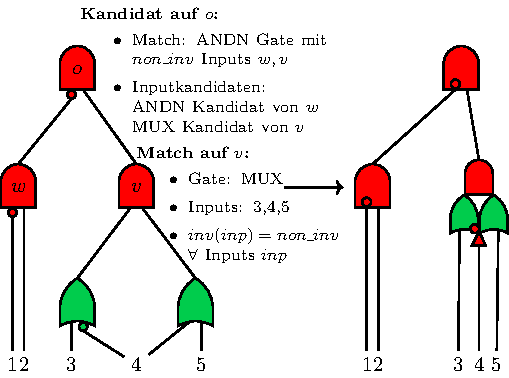
\includegraphics[width = 250pt]{./pictures/compiled/grundl_def_veransch.pdf}
 \caption{Beispiel eines  Kandidaten und eines Matches}
 \label{bild:grundl_definitionen}
\end{center}
\end{figure}

Ein Circuit-Kandidat auf einem Circuit $C$ beschreibt eine mögliche Realisierung der $C$ zugrunde liegenden Funktion.  Wie bereits in der Einleitung dargestellt, gilt es nun den, be\"uglich eines Ma{\ss}es, besten Circuit-Kandidaten auf $C$ zu finden.\\

Wie bereits in der Gate-Definition erwähnt, braucht ein Signal eine gewisse Zeit (Delay) um das Gate zu passieren. Dies gilt ebenfalls für jede Kante eines Circuits. Abhängig von dem Ort der Endknoten und der Lage auf dem Chip besitzt jede Kante einen Delay-Wert der angibt, wie lange ein Signal benötigt um die Kante zu passieren. \\
Des Weiteren ist für die Inputs des Circuits eine Arrivaltime (AT) gegeben die angibt, zu welchem Zeitpunkt das Signal an diesem Input ankommt. Von den Inputs ausgehend lässt sich die Arrivaltime mithilfe der Delay-Werte durch den gesamten Circuit propagieren und entsprechende Werte für die Outputs angeben. Hierbei gilt, dass die Arrivaltime eines Knotens die Ankunftszeit des letzten Signals der Inputs am Output des Knotens angibt. Dies lässt sich auch auf einen Kandidaten übertragen. Dazu folgende Definition:

\begin{definition}{Area und Delay eines Kandidaten:}\\
\label{def:area_delay}
Sei $C$ ein Circuit und $K$ ein Circuit-Kandidat auf $C$, dann gilt: \\
\begin{itemize}
\item $area(K) = \sum_{g \in gates(K)} (area_g + \sum_{i \in inputs(g)} \mathbb{1}_{inv_g(i)} area_{inv})$ 
\item $AT(K) = $\\$  \max\limits_{k \in can(K)} \{\max\limits_{i \in inputs(k)} \{   d_{gate(k)} + \mathbb{1}_{inv_g(i)} d_{inv} + AT(inp\_can(k,i)) + d_{w(k,i)} \} \}$ 
\end{itemize}
Wobei $can(K)$ die Menge der Kandidaten von $K$ ist, $area_{inv}$ die Größe eines Inverters und $inputs(k)$ die Input-Knoten des Output-Knoten des Kandidaten $k$ sind. Des Weiteren ist $d_inv$ das Delay eines Inverters und $d_{w(k,i)} $ das Delay der Kante zwischen den Knoten $k$ und $i$. Hierbei gibt $inp\_can(k,i)$ den Kandidaten des $i$'ten Inputs von $k$ zurück. 
Die $gates(K)$ entsprechen allen durch den Kandidaten $K$ festgelegten Gate-Knoten. 

\end{definition}

\subsection{Kern-Algorithmus}
\label{subsec:kern_algorithmus}

Es folgt ein grundlegender Algorithmus der auf nachfolgend dargestellten eingeschränkten Circuits arbeitet, jedoch im weiteren Verlauf dieser Arbeit zu einer Heuristik für allgemeine sehr große Circuits erweitert wird.

\begin{problem}[framed]{(einfaches) Technology Mapping}
  Instanz:  & Circuit $C$ ohne Multifanoutknoten, mit eindeutigem Output $o$, Library $L$ mit beschr\"anktem $fanin_{max}$\\
  Aufgabe: &  Finde einen Kandidaten $K$ auf $o$, welcher die Arrivaltime/Area minimiert.
\end{problem}

\begin{algorithm}[H]
 \LinesNumbered
 \DontPrintSemicolon
 \caption{(einfaches) Technology Mapping}
 \SetKwInOut{Task}{Task}
 \KwIn{Circuit $C$ kreisfrei mit Output $o$, Library $L$}

 bester\_kandidat[] $\gets \emptyset$\;
 bester\_inv\_kandidat[]$ \gets \emptyset$\;
 \ForEach{Knoten $v \in V(C)$ in topologischer Reihenfolge}
 {
   berechne\_alle\_(invertierten)\_Matche($v$)\;
   \ForEach{ Match $m$ auf $v$ }
   {
      Berechne\_besten\_Kandidaten($m$, $v$)\;
      Update\_best\_(inv)\_kandidat\;
   }
 }
 Implementiere $C$ entsprechend bester\_kandidat[$o$]\;
\end{algorithm}\ \\
\begin{wrapfigure}{r}{2.8cm}
		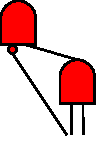
\includegraphics[width = 2.8cm]{pictures/compiled/compl_redundant}
		\caption{Ein Circuit, dessen boolesche Funktion $f = 0 $ ist}
		\label{bild:compl_redundant}
\end{wrapfigure}
Dieser Algorithmus stammt aus \cite{Elbert} und wurde 1987 in \cite{DAGON} entwickelt .\\
Ein \TM (TM) Algorithmus liefert in der Regel nicht die bestmögliche Implementierung der $C$ zugrunde liegenden logischen Funktion. Dies veranschaulicht Abbildung \ref{bild:compl_redundant} welche die Realisierung einer konstanten Funktion darstellt die keine Gates ben\"tigt. Dies ist jedoch mit den bisher eingeführten Möglichkeiten des Technology Mappings nicht möglich. \\

\begin{cor}
	Das einfache \TM  liefert, bezüglich der vorgestellten Möglichkeiten des Matchens und der Kandidatenbildung, den bestmöglichen äquivalenten Circuit.
\end{cor}
\begin{proof} \ \\
	Der Algorithmus geht in topologischer Reihenfolge durch die Knoten $v$ des Graphen und berechnet alle Matche auf $v$. Diese werden dann zu einem Kandidaten ergänzt. 
 Ohne Multifanoutknoten überschneiden sich diese nicht. Für jeden Knoten und jedes Match gibt es nur einen Kandidaten zur Auswahl, da für die Inputs des Matches jeweils nur ein Kandidat gespeichert wurde. An jedem Knoten wird nur das Match, mit dem dazugehörigen Kandidaten, gespeichert, welches die Kosten optimiert. \\
 Es bleibt zu zeigen, dass, angenommen, dass für alle Knoten mit kleinerem topologischen Rang als $rang(v)$ der bestmögliche Kandidat bereits gespeichert ist, so wird, wie soeben dargestellt, auch für $v$ der schnellste bzw. kleinste Kandidat $k$ gespeichert. \\
 Angenommen es gibt einen besseren Kandidaten $k'$, als $k$ welcher von dem Algorithmus gespeichert wurde. Sei $k''$ der Kandidat welcher dasselbe Match wie $k'$ benutzt und die besten Input-Kandidaten. Da $k''$ die besten Input-Kandidaten benutzt, ist er mindestens so schnell (bzw. klein) wie $k'$. Jedoch ist $k$ ebenfalls mindestens so kostengünstig wie $k''$ (andernfalls hätte der Algorithmus $k''$, $k$ vorgezogen). Dies ist ein Widerspruch zur Annahme. 
\end{proof}
 
\begin{cor}{Der Algorithmus für das (einfache) \TM  \\ besitzt $\mathcal{O}(  |V(C)|^3|L|^2)$-Laufzeit}
\end{cor}
\begin{proof}
Schritt 1 und 2 besitzen Laufzeit $\mathcal{O}(1)$. Schritt 4 lässt sich, aufgrund von einem beschränkten $fanin_{max}$ und ohne Multifanoutgates, in $\mathcal{O}(|V(C)|^2|L|)$ errechnen. Der Beweis dieser Aussage befindet sich in Kapitel \ref{subsec:match_kandidaten}.\\
Der Schritt 6 ist schnell implementierbar, da für jeden der max $fanin_{max}$ Inputs der beste Kandidat bereits errechnet wurde und somit nur verlinkt werden muss. Ein invertiertes Match wird nur gebraucht wenn der korrespondierende Input des darüber liegenden Gates invertiert ist. Schritt 6 lässt sich somit in  $\mathcal{O}(fanin_{max})$ realisieren. Schritt 3 und 5 sind zwei verschachtelte Schleifen mit  $|V(C)|$ und $\mathcal{O}(|V(C)|^2|L|)$ Durchläufen. \\
Daraus folgt eine Laufzeit von $\mathcal{O}(  |V(C)|^3|L|)$.
\end{proof}



\section{Entwicklung von FPTAS und Heuristik}
\label{sec:allg_algorithmus}
In diesem Kapitel wird ein Approximationsalgorithmus (ein FPTAS) für allgemeinere Instanzen und Zielfunktionen des Technology Mappings, auf Basis von \cite{Elbert}, vorgestellt. Da auch dieser, um eine polynomielle Laufzeit zu erreichen, noch einige Einschränkungen an gegebene Circuits hat, die für reale Instanzen eines Chips nicht gelten und sich herausstellen wird, dass, nach \cite{ComplexitySynthesis}, das \TM bereits mit einer Konvexkombination als Kostenfunktion  NP-vollständig ist, wird auf Basis des Approximationsalgorithmus eine Heuristik entworfen.

\subsection{Tradeoffprobleme}
\label{subsec:tradeoffprobleme}
Der in Kapitel \ref{subsec:kern_algorithmus} vorgestellte Algorithmus ist in der Lage den bestmöglichen Umbau eines eingeschränkten Circuits bezüglich Area oder Delay zu errechnen. \\
Es existiert  ein Tradeoff zwischen Area und Delay. Dies hat zur Folge, dass ein möglichst kleiner Circuit in der Regel sehr langsam ist und  bei einem schnellen Circuit ein großer Platzverbrauch zu erwarten ist. 
Bei der Lösungsentwicklung mittels \TM  ist jedoch weder ein sehr langsamer noch ein besonders großer Circuit akzeptabel.\\
Daraus folgt die Suche nach einem Algorithmus, welcher in der Lage ist, Circuits  bezüglich einer Konvexkombination oder einer Schranke zu verbessern. Hierbei ergeben sich die beiden folgenden Optimierungsprobleme: 

 \begin{problem}[framed]{\TM mit Konvexkombination}
  Instanz:  & Circuit $C$, mit einem Output, Library $L$ mit beschr\"anktem $fanin_{max}$,
  $|L|$ beschränkt und  Tradeoffparameter $\lambda \in [0,1]$ .\\
  Aufgabe: &  Finde einen Circuit-Kandidaten $K$ auf $C$, welcher $\lambda AT(K) +(1-\lambda )area(K) $ minimiert.
\end{problem}
 \begin{problem}[framed]{\TM mit Arrivaltimeschranke}
  Instanz:  &  Circuit $C$, mit einem Output, Library $L$ mit beschr\"anktem $fanin_{max}$,
  $|L|$ beschränkt und Arrivaltimeschranke $A_{max}$.\\
  Aufgabe: &  Finde den kleinsten Circuit-Kandidaten $K$ auf $C$, für den $AT(K) \leq A_{max}$ gilt oder entscheide, dass für jeden Circuit-Kandidaten $K$ bereits $AT(K) > A_{max}$ gilt.
\end{problem}
In Kapitel \ref{sec:outputs}, werden diese Problemstellungen auf Circuits mit mehreren Outputs erweitert. \\

Beide Probleme lassen sich mit dem noch vorzustellenden FPTAS lösen. Eine Beschreibung, wie sich das \TM mit Arrivaltimeschranke mit dem FPTAS lösen lässt, findet sich in \cite{Elbert}.  Da wie im weiteren Verlauf dieser Arbeit dargestellt, die Arrivaltime nicht der einzige zu beachtende Faktor bei der Geschwindigkeitsoptimierung ist, wird im Folgenden nur noch die Konvexkombination behandelt.\\


Bei der Implementierung eines Algorithmus für die beiden Optimierungsprobleme ergibt sich folgende Herausforderung:\\


Der kosteng\"unstigste Kandidat an einem Knoten $v$ benutzt nicht unbedingt die kosten\"unstigsten Kandidanten der Inputs des Matches von $v$. Es ist n\"amlich m\"oglich, dass einer der Inputs sehr AT kritisch ist und der Subcircuit unter dem anderen Input sehr viel Area ben\"otigt. Dadurch ist es m\"oglich, dass der kosteng\"unstigste Kandidat auf $v$ dem einen Input einen sehr schnellen und dem anderen Input eine sehr kleinen Kandidaten zuweist. Speichert man an jedem Knoten nur den kostenminimierenden noch vorhandenen Kandidaten, bleibt somit keine Garantie, dass der kosteng\"unstigste Circuit-Kandidat am Output noch vorhanden ist.\\

Die Kosten eines Kandidaten $k$ sind aus diesem Grund nicht $\lambda AT(k) +(1-\lambda )area(k)$,  sondern das Tupel $(AT(k), area(k))$.
Es gibt jedoch eine Klasse von Kandidaten, welche nicht gespeichert werden muss. Hierzu die folgende Definition:

\begin{definition}{(dominierte Kandidaten)}\\
	Seien $k_1, k_2$ Kandidaten desselben Knotens. Dann wird $k_2$ von $k_1$ dominiert wenn mindestens eine der folgenden Bedingungen erfüllt ist:
	\begin{itemize}
	\item $AT(k_1) < AT(k_2) \text { und  }area(k_1) \leq area(k_2)$
	\item $	AT(k_1) \leq AT(k_2) \text{ und } area(k_1) < area(k_2)$	
	\end{itemize}
\end{definition}

 \begin{wrapfigure}{r}{6cm}
		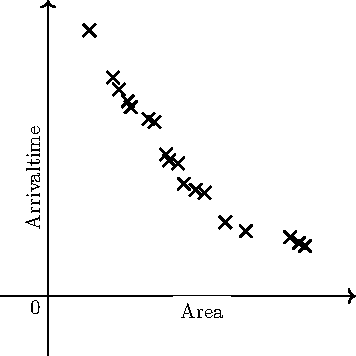
\includegraphics[width = 6cm]{pictures/compiled/tradeoff_kurve}
		\caption{Ordnen der Kandidaten in einer Tradeoffkurve}
		\label{bild:tradeoff_kurve}
\end{wrapfigure}
Eine optimale Lösung des Technology Mappings verwendet nur nicht-dominierte Kandidaten.
Angenommen dies wäre nicht der Fall, ließe sich durch Ersetzen eines dominierten durch einen nicht dominierten Kandidaten eine bessere Lösung erzielen; dies ist jedoch ein Widerspruch zu Optimalität der Lösung.\\
Daraus folgt, dass nur die nicht-dominierten Kandidaten während der Ausführung des Algorithmus gespeichert werden müssen.\\
Die Menge der noch bleibenden Kandidaten lassen sich in einer sogenannten Tradeoff-Kurve speichern (s. Abb. \ref{bild:tradeoff_kurve}), die jeden Kandidaten zweidimensional anhand seiner Kosten erfasst.\\

Die beiden vorgestellten Probleme sind NP-vollständig. Ein Beweis dieser Aussage und genauere Informationen zur Einordnung der Schwere dieser Probleme finden sich in \cite{ComplexitySynthesis} und \citep{Elbert}. \\
Daraus folgt, dass sich ab diesem Punkt wahrscheinlich  kein polynomieller Algorithmus für das \TM finden lässt, der, hinsichtlich der vorgestellten Operationen des Technology Mappings, den kostengünstigsten Circuit-Kandidaten liefert.\\
Da bei zwei nicht dominierenden Kandidaten nicht eindeutig ist, welcher der bessere ist,  wird eine Vielzahl von Kandidaten an jedem Knoten gespeichert. Dies zeigt sich in einem exponentiell großen Speicherbedarf. 

\subsection{Multifanoutknoten}
\label{subsec:multifanout}
 \begin{wrapfigure}{r}{6cm}
		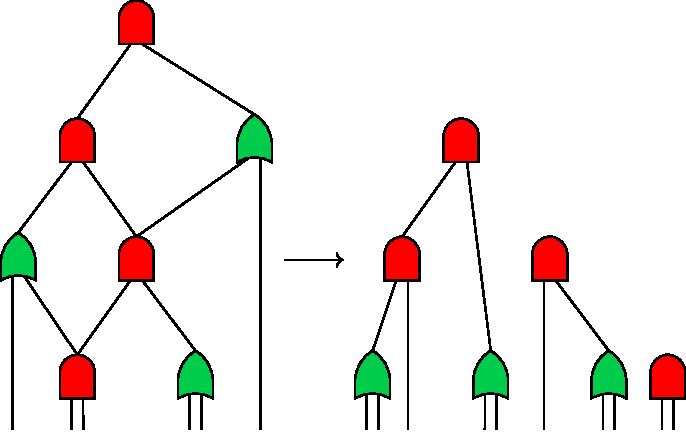
\includegraphics[width = 6cm]{pictures/compiled/ohne_highfanout_heu}
		\caption{Unterteilen eines Circuit in Multifanoutfreie Subcircuits}
		\label{bild:ohne_multifanout_heu}
\end{wrapfigure}
Der beschriebene Kern-Algorithmus arbeitet nur auf Circuits, in denen keine Multifanoutknoten existieren. Diese kommen auf einem realen Chip jedoch zu ca. $30\%$ vor.
Eine Analyse über die Auswirkungen von der Anzahl der Multifanoutknoten auf die Laufzeit des Algorithmus befindet sich Kapitel \ref{sec:analyse}.\\

Es ist möglich einen Circuit in kleinere Subcircuits zu unterteilen, die solche Multifanoutknoten nicht beinhalten. Diese Subcircuits werden einzeln mit dem Algorithmus (sehr schnell) optimiert und daraufhin zu einem C äquivalenten Circuit C' zusammengesetzt. Diese Vorgehensweise findet sich ausführlich in \cite{DAGON} wieder. Abbildung \ref{bild:ohne_multifanout_heu} stellt diesen Ansatz einer Heuristik dar. \\
   \begin{wrapfigure}{r}{7cm}%[htb]
%\centering
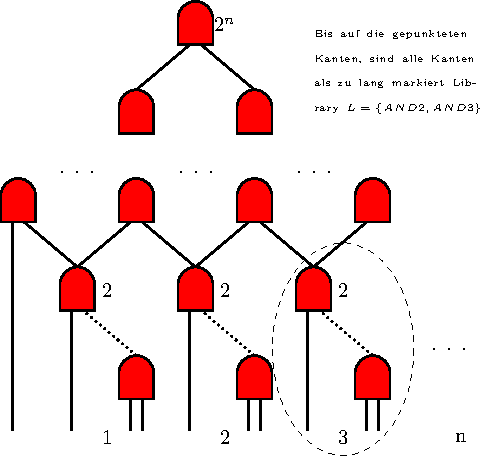
\includegraphics[width= 7cm]{pictures/compiled/expo_kand}
\caption{Exponentiell viele Kandidaten bereits bei sehr eingeschränkter Library}
\label{bild:expo_kan}
\end{wrapfigure}
  Der Anteil an Multifanoutknoten ist auf den mir vorliegenden Chips so groß, dass eine Vielzahl sehr kleiner Subcircuits entstehen, woraus folgt, dass die Möglichkeiten des Technology Mappings sehr eingeschränkt werden. 

Aus diesem Grund werde ich diesen Weg einer Heuristik nicht weiter verfolgen.

Bei der Implementierung von Multifanoutknoten besteht die größte Herausforderung darin, dass bei der Konstruktion des äquivalenten Circuits die eingebauten Kandidaten aller Nachfolger eines Multifanoutknoten $v$ an $v$ übereinstimmen müssen. Daraus folgt, dass bei der Wahl eines Kandidaten für einen Knoten $w$, die  Input-Kandidaten von $w$, nicht unabhängig voneinander gewählt werden können. \\

Abbildung \ref{bild:expo_kan} zeigt zudem eine weitere Herausforderung für die Implementierung auf. Die Anzahl der zu speichernden Kandidaten kann  exponentiell bezüglich $|V(C)|$ sein. Zum Beispiel liegen am Output des Citcuits dieser Abbildung mindesten $2^n$ verschiedene Kandidaten vor, da am Output des gepunkteten Subcircuits  2 Kandidaten vorhanden sind und dieser Subcircuit $n$ mal in dem Graphen vorkommt. Die Anzahl der Knoten in dem Graphen ist polynomiell in $n$.  \\
Zur Lösung der ersten Herausforderung helfen die folgenden Definitionen:\\

\begin{definition}{Cone eines Knoten:}\\
	Sei C ein Circuit und v ein Knoten von C dann sei die Cone von v: 
	\[ cone(v) := C[V \cup \{ v \}], V = \{ w \in V(C) : \exists \text{ w-v-Weg in }  C \} \] 
	Die durch die $cone(v)$ berechnete logische Funktion wird die	{\bf bis v berechnete Funktion} genannt.
\end{definition}

\begin{definition}{Offene Knoten:}\\
	Sei $C$ ein Circuit und $v,w \in V(C)$, dann heißt $o$ offener Knoten von $v$, wenn Folgendes gilt: 
	\begin{itemize}
		\item $ o \in cone(v)\backslash \{ v \} $
		\item $| \delta ^{+}(o)| \geq 2$
		\item $ \exists w \in V(C) \backslash cone(v) : \exists \text{ o-w-Weg in } C \text{ ohne v} $
	\end{itemize}	
\end{definition}
 \begin{wrapfigure}{r}{5.5cm}
		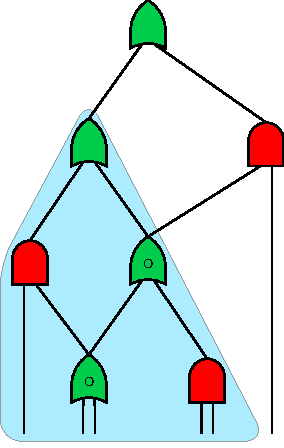
\includegraphics[height = 7cm]{pictures/compiled/cone}
		\caption{Visualisierung der Definitionen 3.2 und 3.3}
		\label{bild:cone}
\end{wrapfigure}
Somit ist die Menge der offenen Knoten eines Circuit Knoten $v$ die Menge aller Multifanoutknoten $o$, von welchen aus man sowohl $v$ als auch einen Knoten außerhalb der Cone von $v$ erreichen kann. In dieser Menge ist $v$ selber nicht enthalten. Die offenen Knoten von $v$ sind gerade die Multifanoutknoten, die durch die Kandidaten eines Knotens außerhalb von $cone(v)$ verändert werden können. Alle Kandidaten von  Knoten mit Ausgangsgrad 1 und dieser Eigenschaft sind durch den Nachfolger-Kandidaten, der auch zu einem offenen Knoten gehören muss, bereits eindeutig definiert. \\
Abbildung \ref{bild:cone} visualisiert die vorangegangenen Definitionen. Hierbei entsprechen die  mit o markierten Knoten den offenen Knoten der $cone(v)$.

\begin{definition}{Klasse eines Kandidaten:}\\
	Sei $k$ ein Kandidat auf einem Knoten $v$ und $O$ die Menge der offenen Knoten von $v$. Die Klasse $class(k)$ ist eine Abbildung, welche jedem Element $w \in O$ den durch $k$ festgelegten Kandidaten auf $w$ zuordnet.
\end{definition}
Hiernach lassen sich zwei Kandidaten $k_1,k_2$ eines Knoten $v$ mit $class(k_1) \neq class(k_2)$ nicht miteinander vergleichen. Dies gilt auch für den Fall wenn $k_2$ von  $k_1$ dominiert wird, denn es ist möglich, dass dies zwar an der Stelle $v$ gilt, jedoch nicht an allen offenen Knoten von $v$. Daraus folgt, würde man $k_2$ löschen, so löscht man evtl. den besten Kandidaten des Outputs von $C$. \\
Um daher mit Multifanoutknoten arbeiten zu können, werden für jeden Knoten $v$ und jede Klasse von $v$ alle nicht dominierten Kandidaten gespeichert. Dann ist der noch verbleibende beste Kandidat des Outputs die beste Lösung. Dies führt jedoch zu einem nur exponentiell beschränkten Speicheraufwand.\\
Zur Speicherung der Kandidaten wird für jede Klasse eines Knotens eine Tradeoff-Kurve angelegt.

\subsubsection{Klonen}\label{subsubsec:klonen}
Die Input-Kandidaten eines Kandidaten müssen aus nachfolgend dargestelltem Grund an deren offenen Knoten übereinstimmen:\\
Angenommen dies wäre nicht der Fall dann würden offene Knoten evtl. mehrere Male mit verschiedenen Kandidaten gebaut. Dieser Vorgang wird auch Klonen genannt. Dies kann von Vorteil sein, wenn zum Beispiel ein offener Knoten Teil eines sowohl sehr Delay- als auch sehr Area-kritischen Gebietes ist. Dann würde einmal ein schneller und einmal ein sehr kleiner Kandidat realisiert. Dies führt in der Regel jedoch zu einem deutlich erhöhten Platzverbrauch und es werden mehr Kanten gebraucht, was ich vermeide. Die erhöhte Anzahl an Kanten bringt höhere Routing Kosten mit sich, welche im \TM jedoch nicht berücksichtigt werden. Um zu verhindern, dass nicht beachtete Ressourcen übermäßig verbraucht werden, ist das Klonen in den vorgestellten Algorithmen nicht erlaubt und wird durch die Klassen und die Routine, welche beim Verknüpfen von Input-Kandidaten zu einem neuen Kandidaten genutzt wird, verhindert. 

\subsection{Zu lange Kanten}
\label{subsec:zu_lange_kanten}
 \begin{wrapfigure}{r}{6cm}
		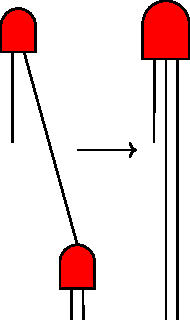
\includegraphics[height = 8cm]{pictures/compiled/zu_lange_kante}
		\caption{Visualisierung eines Matches über eine lange Kante}
		\label{bild:zu_lange_kanten}
\end{wrapfigure}
Abbildung \ref{bild:zu_lange_kanten} veranschaulicht eine häufig auftretende Situation. Es handelt sich um das Matchen über eine auf dem Chip sehr lange Kante. Dadurch verbessert sich evtl. die Größe des Circuits, jedoch sind nach dem Match nun zwei sehr lange Kanten auf dem Chip vorhanden, was einen großen Routing-Aufwand und weitere Kosten mit sich bringt und somit eine zu vermeidende Situation ist. \\
In Kapitel \ref{subsec:mehrere_outputs} wird eine zusätzliche Klasse von Kanten eingeführt, über welche man nicht matchen darf.
Diese Kanten bezeichnet man als konstant.
Deshalb wird bei der Bildung eines jeden Matches darauf geachtet über keine konstante Kante zu matchen.\\
Durch das Hinzufügen der zu langen Kanten zu den konstanten Kanten kann keine optimale Lösung mehr im Kern-Algorithmus garantiert werden, denn es ist möglich, aber unwahrscheinlich, dass die zusätzlichen Routing-Kosten vernachlässigbar sind und ein Match über diese Kante für eine optimale Lösung notwendig ist. \\

 \subsection{Teilweise überflüssige Subcircuits}
 \label{subsec:teilweise_ueberfkl_subcircuits}
 Abbildung 4 zeigt, dass nicht unbedingt alle Inputs eines Circuits relevant sind für die Outputs. Zur genaueren Einordnung folgt eine Definition:
 
 \begin{definition}{Vollständig überflüssiger und teilweise überflüssiger Circuit }
 	Sei $C$ ein Circuit mit logischer Funktion $ f : \{ 0 , 1 \}^n \rightarrow \{ 0 , 1 \}^m $.\\
 	$C$ wird vollständig überflüssig genannt wenn gilt:
 	\[  \exists y \in \{0,1 \}^m :\forall x \in \{ 0, 1\}^n : f(x) = y  \]
 	$C$ wird teilweise überflüssig genannt wenn es eine Teilmenge der Inputs gibt, von denen die Signale der Outputs nicht abhängen.
 \end{definition}
 
Die Berücksichtigung von vollständig überflüssigen Subcircuits würde bedeuten, dass Teile des Circuits entfernt werden und die nun freien Pins der nachfolgenden Knoten an permanenten Strom gelegt oder mit der Erdung des Chips verbunden werden müssen. Dies lässt sich jedoch weiter optimieren. Da die Information an den nachfolgenden Gates vorhersagbar ist, muss sie auch nicht verarbeitet werden. Daraus folgt eine hohe Einsparung von Kosten. Es bedingt jedoch ebenfalls einen großen Aufwand zur Implementierung in die aktuelle Architektur des \TM Algorithmus. In der Praxis ist das Vorkommen von  vollständig überflüssigen Subcircuits verschwindend gering. Von daher werden die vollständig überflüssigen Subcircuits in dieser Arbeit nicht weiter behandelt und kommen in der Implementierung der noch folgenden Algorithmen nicht vor. \\
 
Im Gegensatz dazu kommen die teilweise überflüssigen Circuits durchaus vor. Bei der Konstruktion eines Chips geschieht dies durch das Zusammensetzen unterschiedlicher Circuits.\\
 \begin{wrapfigure}{r}{6cm}
		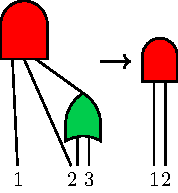
\includegraphics[height = 5cm]{pictures/compiled/partly_redundant}
		\caption{Nur Input 1 und 2 sind die relevanten Inputs}
		\label{bild:partly_redundant}
\end{wrapfigure}
In den meisten Fällen werden die teilweise überflüssigen Circuits automatisch bei der  Suche der Matche gefunden, da die irrelevanten Inputs nicht mehr unter den Inputs des Match auftauchen und somit beim Bau des äquivalenten Graphen verschwinden. Dies veranschaulicht Abbildung \ref{bild:partly_redundant}. \\
Es gibt dabei jedoch noch eine Besonderheit. Wenn alle Inputs bis auf einen irrelevant sind, so ist das resultierende Gate des Matches entweder ein Inverter(INV) oder ein Buffer(BUFF). Ersteres lässt sich als Input-Invertierung des darüberliegenden Input-Pins speichern. Ein Buffer ist jedoch nicht unbedingt in der Library für das \TM vorhanden und kann vermieden werden, indem kein Buffer, sondern nur die Kanten vom Input des Buffers zu seinen Outputs gebaut werden. Dies verhindert den Einbau eines nicht nötigen Gates. Da $fanout_{max}$ und $fanin_{max}$ im weiteren Verlauf dieser Arbeit beschränkt werden, lässt sich dies in linearer Laufzeit implementieren. Diese zusätzliche Bearbeitung läuft dann in jedem folgenden Algorithmus automatisch im Hintergrund und findet keine Erwähnung mehr.\\
 Obwohl nun das Gegenbeispiel aus Kapitel \ref{subsec:kern_algorithmus} nicht mehr gültig ist, lässt sich mit den Möglichkeiten des Technology Mappings in der Regel keine optimale Realisierung der des Circuits zugrunde liegenden logischen Funktion finden.
 
 
\subsection{Match-Probleme}
\label{subsec:match_kandidaten}
In Circuits mit beliebig vielen Multifanoutknoten steigt die Anzahl der möglichen Matche eines Knotens sehr stark an, was eine direkte Auswirkung auf die Größe der Menge der möglichen Kandidaten hat. \\
Es folgt eine weitere Betrachtung von Matches und daraus ableitend ein Algorithmus der auf Instanzen von real existierenden Chips fast alle möglichen Matche findet und in polynomieller Zeit implementierbar ist.

\subsubsection{Obere Schranke für die Anzahl Matche eines Knoten}
\label{subsubsec:anzahl_matchings}
Folgendes Lemma legt eine äquivalente Definition für Matche nahe.
Sei ein Circuit $C$ ohne teilweise überflüssige Subcircuits gegeben: \\$\bar{C}_v := (V(C[cone(v)]), \{ (u,w) | (w,u) \in E(C[cone(v)])\})$.
\begin{lemma}{Die Inputs eines Matches auf $v$ lassen sich eindeutig zu den Kanten einem gerichteten $v$-Schnitts in $\bar{C}_v $} zuordnen.
\end{lemma}
\begin{proof}
Zu jedem Inputpin eines Matches gehört eindeutig eine Kantenmenge $K$ aus $C$. Es ist möglich, dass $|K| > 1$, denn ein Match kann mehrere ausgehende Kanten eines Knoten zu einer Kante zusammenfassen. Dies veranschaulicht Abbildung \ref{bild:mux_match} für ein Match eines MUX Gates.  Sei $I$ die Menge der mit den Inputs korrespondierenden Kantenmengen.\\
Es genügt zu zeigen, dass alle Kanten $I'$ in $I$ gerade die Kantenmenge eines gerichteten $v$-Schnitts in $\bar{C}_v$ sind. \\
Angenommen $I'$ bildet keinen gerichteten $v$-Schnitt, dann existiert in $\bar{C}_v\backslash I$ ein Weg von einem Input von $cone(v)$ zu $v$, welcher keine Kante aus $I$ benutzt. \\
Eine Kante dieses Weges muss jedoch zu einem der Inputs des Matches gehören, denn sonst hätte das Match einen Seiteninput, was nicht erlaubt ist oder es existiert ein teilweise überflüssiger Subcircuit. 
\end{proof}

\begin{wrapfigure}{r}{6cm}
		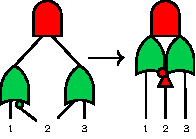
\includegraphics[width = 6cm]{pictures/compiled/mux_match}
		\caption{Das MUX Match verbindet zwei Kanten eines Multifanoutknoten}
		\label{bild:mux_match}
\end{wrapfigure}

Anhand eines Schnitts kann nicht eindeutig hergeleitet werden, ob mehrere Kanten eines Outputs zusammengefasst oder getrennte Input-Kanten eines Matches sind. Dies wird ebenfalls durch Abbildung \ref{bild:mux_match} veranschaulicht. Ohne Multifanoutknoten ist diese Zuweisung jedoch, abgesehen von den möglichen Invertierungen der Inputs und des Outputs, eineindeutig wenn es keine zwei Gates der Library gibt, welche die gleiche  logische Funktion realisieren.\\
In einem Graphen ohne Multifanoutknoten gilt somit: \\
Die Menge der Matche von $v$ ist somit gerade die Menge aller maximal $fanin_{max}$ großen $v$-Schnitte in $\bar{C}_v$, inklusive aller möglicher Inputinvertierungen und Outputinvertierungen, die als Subgraph die logische Funktion eines Gates der Library realisieren.
\begin{cor}\label{cor:anz_matche_einfach}
Sei $C$ ein Circuit ohne teilweise überflüssige Subcircuits. Die Anzahl der Matche eines Knotens $v\in V(C)$ mit $m_v := |E(C[cone(v)]|$, wobei $C[cone(v)]$ keine Multifanoutknoten enthält, ist durch $m_v^{fanin_{max}} 2^{fanin_{max}+1} fanin_{max}$ beschränkt.
\end{cor}
\begin{proof}
Sei  $X_v:= \{ E \subseteq E(C[cone(v)]) | |E|\leq fanin_{max}  \}$. Die Menge der maximal $fanin_{max}$ großen $v$-Schnitte ist in $C[cone(v)]$ durch $ |X_v|$ beschränkt. Es gilt hierbei:
\[ |X_v| = \sum\limits_{i \leq fanin_{max}} \binom{m_v}{i} \leq  \sum\limits_{i \leq fanin_{max}}\frac{m_v!}{i!(m_v-fanin_{max})!} \leq m_v^{fanin_{max}} fanin_{max} \]
Für jeden Schnitt gibt es zwei verschiedene mögliche Output-Invertierungen und maximal  $2^{fanin_{max}}$ viele Möglichkeiten die Inputs zu invertieren. Jedes mögliche Match ist nun durch ein Element aus $X_v$ und eine Wahl von Invertierungen eindeutig charakterisiert.
\end{proof}
Für allgemeinere Circuits lässt sich folgende Schranke angeben: 
\begin{cor}\label{cor:anzahl_matche_bel}
Sei $C$ ein Circuit ohne teilweise überflüssige Subcircuits. Die Anzahl der Matche eines Knotens $v\in V(C)$ mit $m_v := |E(C[cone(v)]|$, ist durch \\ $m_v^{fanin_{max}} fanin_{max}^22^{fanin_{max}+1}2^{fanout_{max}}$ beschränkt.
\end{cor}
\begin{proof}
Korollar \ref{cor:anz_matche_einfach} gibt eine obere Schranke für die Anzahl aller Matche inklusive der möglichen Invertierungen für einen Circuit ohne Multifanoutknoten an. Sei $u \in x \in X_v$ (Definition siehe oben) ausgehende Kante eines Multifanoutknoten $w$, so gibt es bis zu $2^{fanout_{max}-1}$ Möglichkeiten weitere Kanten von $w$ der korrespondierenden Kantemenge von $u$ hinzuzufügen.  Diese Möglichkeit besteht für alle maximal $fanin_{max}$ Kanten von $x$. Durch Multiplikation mit der oberen Schranke aus Korollar \ref{cor:anz_matche_einfach} folgt die Aussage.
\end{proof}
In einem Circuit ohne Multifanoutknoten lässt sich die Schranke noch genauer angeben. 
\begin{cor}\label{cor:anz_matche_einfach_genauer}
Sei $C$ ein Circuit ohne Multifanoutknoten. Die Anzahl der Matche eines Knoten ist durch $2^{2fanin_{max} +1}fanin_{max}$ beschränkt.
\end{cor}
\begin{proof}
Ausgehend von einem Knoten $v \in V(C)$ mit maximal $fanin_{max}$ Inputs gibt es  $2^{fanin_{max}}$ Möglichkeiten, die an den Inputs liegenden Gates mit in das Match einzuschließen. Bis auf eine schließt jede dieser Möglichkeiten mindestens ein Gate mit ein. Da $C$ keine Multifanoutknoten enthält, wird der Fanin des Matches um mindestens eins erhöht, denn es ist nicht möglich, Kreise zu schließen. Daraus folgt, dass dieser Schritt maximal $fanin_{max}$ mal durchführbar ist. Für jeden so berechneten Prototyp einen Matches gibt es noch $2^{fanin_{max}}$ mögliche Invertierungen der Inputs und $2$ des Outputs, woraus die obige Aussage folgt.
\end{proof}
\begin{definition}
Sei $\mathcal{M}:= |V(C)|^{fanin_{max}} fanin_{max}^22^{fanin_{max}+1}2^{fanout_{max}}$ eine Bezeichnung der oberen Schranke für die Anzahl der Matche eines Knotens in einem Graphen mit beschränktem $fanin_{max}$ und $fanout_{max}$.
\end{definition}

\subsubsection{Match-Suche in polynomieller Zeit}
\label{subsubsec:pol_match_suche}
Der Kern-Algorithmus aus Kapitel \ref{subsec:kern_algorithmus} findet alle möglichen Matche eines beliebigen Knotens in polynomieller Zeit, da in dem Circuit keine Multifanoutknoten existieren. Aus Korollar \ref{cor:anz_matche_einfach_genauer} folgt, dass potenzielle Matche aller Knoten  in $\mathcal{O}(2^{2fanin_{max} +1}fanin_{max} |V(C)|)$ errechnet werden können. Da $fanin_{max}$ als Konstante deklariert wurde, entspricht dies linearer Laufzeit. Es bleibt zu prüfen, ob  ein solcher Prototyp einem Match in $C$ entspricht, also ob die logische Funktion des Subcircuits einem Match der Library gleicht. Für jede der maximal $2^{fanin_{max}}$ möglichen Wahrheitsbelegungen der Inputs wird der Wahrheitsgehalt des Outputs errechnet. Dies ist linear in $|V(C)|$ möglich. Die dadurch errechnete Tabelle wird mit den $|L|$ Gates der Library verglichen. \\
Daraus folgt, dass das Finden aller Matche in $\mathcal{O}(|V(C)|^2|L|)$ erfolgt und somit polynomiell möglich ist.

Bei Circuits mit beliebig vielen Multifanoutknoten, aber beschränktem $fanout_{max}$, lassen sich nach Korollar \ref{cor:anzahl_matche_bel} und gleichem Vorgehen, wie soeben beschrieben, alle Matche ebenfalls in polynomieller Zeit finden. Dabei beträgt die Laufzeit $\mathcal{O}(|V(C)|^{fanin_{max}+2}|L|)$.

\subsubsection{Heuristische Match-Suche}
In der Praxis wird, ähnlich der Routine ohne Multifanoutknoten, von dem Gate eines Knotens ausgehend überprüft, ob dieser oder eine mögliche Invertierung der Inputs und des Outputs einem Gate der Library entspricht. 

Es gibt maximal $2^{fanin_{max}}$ Möglichkeiten, das potenzielle Match mit den an den Inputs liegenden Gates zu erweitern. Für jede dieser Möglichkeiten wird ein weiteres potenzielles Match gebildet und mit jeder möglichen Invertierung der Inputs und des Outputs überprüft ob es einem Match entspricht.
Dieser Vorgang wird für jede der Möglichkeiten so lange wiederholt, bis die Anzahl der Inputs des, durch das potenzielle Match beschriebenen, Subcircuits größer als $fanin_{max}$ ist. Ab diesem Punkt wird das vorliegende potenzielle Match nicht mehr erweitert. \\
Bei einem Circuit mit Multifanoutknoten kann hierdurch jedoch das Finden aller möglicher Matche nicht sichergestellt werden, da sobald ein potenzielles Match einen Multifanoutknoten mit einschließt, die Zahl der Inputs sinken kann. \\
In der Praxis werden so jedoch die überwiegende Mehrheit der Matche gefunden. Der Verlust einiger weniger Matche ermöglicht jedoch einen enormen Laufzeitgewinn.
Eine genaue Beschreibung dieser Routine findet sich in \cite{BooleanMatching}. Diese Routine wird auch Boolean Matching genannt.

\subsection{Kandidaten-Probleme}
\label{subsec:kand_prob}
Die Anzahl der Kandidaten an einem Knoten ist im Allgemeinen nicht polynomiell beschränkt wie Abbildung \ref{bild:expo_kan} beweist. Dies gilt offenbar auch wenn der Circuit $C$ keine Multifanoutknoten hat. Dieses Problem wird durch das Filtern mit Buckets in Kapitel \ref{subsubsec:filtern} gelöst.

\subsubsection{Schranken für Arrivaltime und Größe}
\label{subsubsec:schrankenalgo}
Zur Vorbereitung auf das Filtern mit Buckets wird folgender Algorithmus eingeführt.\\
Für die Bearbeitung einer Tradeoffkurve ist es notwendig Schranken angeben zu können, zwischen welchen sich alle Werte der Kurve befinden, damit sich nach dem Filtern in Kapitel \ref{subsubsec:filtern} die Anzahl der noch vorhandenen Kandidaten abschätzen lässt. \\
Durch den vorhandenen Tradeoff befindet sich die $AT$ eines Circuits $C$ zwischen der schnellsten und der kleinsten Implementierung von $C$. Dementsprechend befindet sich $Area$ von $C$ zwischen der kleinsten und schnellsten Lösung. Folgender Algorithmus, der in \cite{Elbert} entwickelt wurde, nähert die entsprechenden Circuit-Kandidaten an.\\

\begin{algorithm}[H]
 \LinesNumbered
 \DontPrintSemicolon
 \caption{Untere Schranke Arrivaltime}
 \SetKwInOut{Task}{Task}
 \KwIn{Circuit $C$, Library $L$}

 schnellster\_kandidat[] $\gets \emptyset$\;
 schnellster\_inv\_kandidat[]$ \gets \emptyset$\;
 \ForEach{Knoten $v \in V(G)$ in topologischer Reihenfolge}
 {
   berechne\_alle\_(invertierten)\_Matche($v$)\;
   \ForEach{ Match $m$ auf $v$ }
   {
      berechne\_schnellsten\_Kandidaten($m$,$v$)\;
      Update schnellster\_(inv)\_kandidat\;
   }
   \If{ $v$ ist Multifanoutknoten }
   {
      
      \If{ schnellster\_kandidat[v].AT $<$ schnellster\_inv\_kandidat[v].AT }
      {
	l\"osche schnellster\_inv\_kandidat[v]\;
      }
      \Else
      {
	l\"osche schnellster\_kandidat[v]\;
      }
   }
 }
 Baue $C'$ entsprechend schnellster\_kandidat[$o$]\;
 \Return $C'$\;
\end{algorithm}\ \\

Dieser Algorithmus führt den Kern-Algorithmus  auf $C$ aus und behält für jeden Knoten nur einen Kandidaten. Dadurch ist es nicht notwendig mehr als $|V(C)|$ Kandidaten zu speichern. \\
 Die untere Schranke für Area wird mit einem entsprechenden Algorithmus berechnet. \\
Im Gegensatz zu dem Kern-Algorithmus garantiert dieser keine optimale Lösung bezüglich Arrivaltime oder Area, da es möglich ist, dass für einen Knoten $v$ und einen seiner Inputs $i$ der schnellste bzw. kleinste Kandidat auf $v$ eine Invertierung an $i$ vorsieht. Da der beste Kandidat mit invertiertem Output von $i$ evtl. in Schritt 10  oder 12 gelöscht wurde, ist der optimale Kandidat für $v$ möglicherweise nicht mehr vorhanden. Der Unterschied zum Kern-Algorithmus liegt darin, dass für $i$ die besten Kandidaten beider Invertierungen gespeichert werden. Da $i$ hier jedoch evtl. ein Multifanoutknoten ist, würde dies zu einem Verlust der Polynomialität führen.\\

Unter welchen Bedingungen sich dieser Algorithmus polynomiell implementieren lässt, wird in Kapitel \ref{subsec:heuristik} weiter ausgeführt. Dort wird dieser Algorithmus mit der Laufzeit der Heuristik ohne diese Routine beschrieben. Da jedoch nur maximal zwei Kandidaten an jedem Knoten gespeichert werden und alle Matche nur einmal gefunden werden müssen, wird die Laufzeit der Heristik mit der Hinzunahme dieses Algorithmus nur geringfügig beeinflusst.\\

\subsubsection{Filtern mit Buckets}
\label{subsubsec:filtern}
Die Kandidaten eines beliebigen Knotens sind in Tradeoffkurven, nach Klassen sortiert, gespeichert. Die Werte einer solchen Kurve lassen sich in Abschnitte (Buckets) fester Größe einteilen. Dabei lässt sich eine Kurve sowohl in Delay-Buckets  der Größe $\delta_{delay}$ als auch in Area-Buckets der Größe $\delta_{area}$ unterteilen. Dies wird in Abbildung \ref{bild:tradeoff_kurven_filtern} veranschaulicht. Diese und Abbildung \ref{bild:tradeoff_kurve} wurden \cite{Elbert} entnommen. \\

Ziel dieses Kapitels ist es, die maximale Anzahl von Kandidaten in jeder Kurve zu beschränken, unter der Voraussetzung, dass die Güte des resultierenden Circuit-Kandidaten nur um einen Faktor $\epsilon > 0$ von der optimalen Lösung entfernt ist, mit dem Vorteil diese Lösung in polynomieller Zeit berechnen zu können. 
\begin{figure}[h]
\centering
\begin{subfigure}{.5\textwidth}
  \centering
  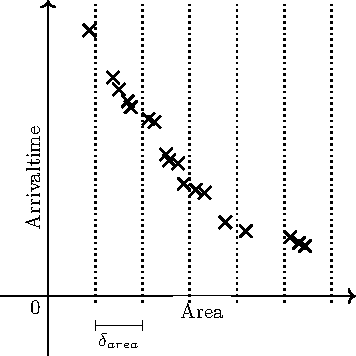
\includegraphics[width=.7\linewidth]{pictures/compiled/tradeoff_kurve_buckets}
\end{subfigure}%
\begin{subfigure}{.5\textwidth}
  \centering
  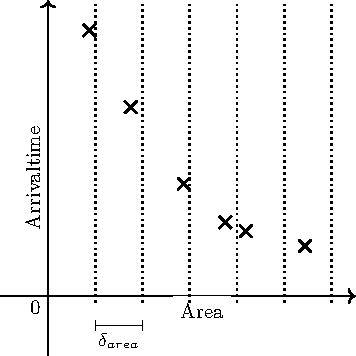
\includegraphics[width=.7\linewidth]{pictures/compiled/tradeoff_kurve_filtered}
\end{subfigure}
\caption{Einteilen und Filtern mit Buckets}
\label{bild:tradeoff_kurven_filtern}
\end{figure}

Man wählt die Bucketgrößen $\delta_{delay} = \frac{\epsilon X^{-}}{2n\lambda}, \delta_{area} = \frac{\epsilon X^{-}}{2n(1-\lambda)}$ (mit Tradeoff $\lambda$ und Approximationsfaktor $\epsilon$ ), und speichert erst nur den kleinsten Kandidaten in jeder Area-Bucket und von den verbleibenden nur den schnellsten in jeder Delay-Bucket. Hierbei entspricht $X^-$ der mit dem Untere Schranke Area Algorithmus errechneten Schranke und $n$ der Anzahl der Knoten des Circuits. \\
Für $\lambda \in \{ 0,1 \}$ ist jeweils eine der Bucketgrößen nicht definiert. In diesem Fall wird für den nicht definierten Fall nur der beste Kandidat (schnellster bzw. kleinster) behalten; d.h. im nicht definierten Fall die Tradeoffkurve in nur ein Bucket unterteilt.\\
Die maximale Anzahl an Kandidaten in einer Tradeoffkurve ist nach dem Filtern polynomiell beschränkt. 
Filtert man jede Tradeoffkurve wie beschrieben, ist der noch bestmögliche Circuit Kandidat nur um den Faktor $\epsilon$ von der optimalen Lösung entfernt. Ein Beweis dieser Aussage befindet sich in \cite{Elbert}.
\begin{definition}
Sei $\mathcal{B}$ die maximale Anzahl an Kandidaten in einer Tradeoffkurve nachdem sie gefiltert wurde.\\
Des Weiteren sei $\mathcal{K}$ die maximale Anzahl von Klassen eines Knotens.
\end{definition}
\begin{cor}\label{cor:anzahl_klassen}
Für Circuits $C$ mit konstanter Anzahl $k$ an Multifanoutknoten sind $\mathcal{B}$ und $\mathcal{K}$ polynomiell beschränkt.
\end{cor}
\begin{proof}
$\mathcal{B}$ ist beschränkt durch die Größe des größtmöglichen äquivalenten Circuit $C_A$ von $C$ geteilt durch $\delta_{area}$. Sei $X^+$ eine mit dem Algorithmus: Untere Schranke Arrivaltime errechnete obere Schranke für die Größe von $C$. Daraus folgt $\mathcal{B} \in \mathcal{O}(X^+ \cdot \frac{2n(1-\lambda)}{X^- \epsilon})$. $\mathcal{B} $ ist somit polynomiell in $\frac{X^+ n}{X^- \epsilon}$. 



Da die Größe $area_{max}$ (Delay) des größten (langsamsten) Gates der in Abbildung \ref{bild:new_library} beschriebenen Library weniger als einen Faktor 10 größer (langsamer), als die entsprechenden Werte des kleinsten (schnellsten) Gates dieser Library, ist folgt, dass $\frac{X^+ n}{X^- \epsilon}$ polynomiell beschränkt ist.  Der größtmögliche zu $C$ äquivalente Circuit ist nämlich nicht größer als $|V(C)|(fanin_{max}+1)area_{max} + |O|area_{max}$. Die Größe jedes Gates mit möglichen Invertern an seinen Inputs in $C$ ist durch $(fanin_{max}+1)area_{max}$ beschränkt und die Anzahl der an den Outputs $O$ liegenden Inverter durch $|O|$.\\
Für eine allgemeine Library findet sich in \cite{Elbert} eine Lösung zur Erhaltung der Polynomialität.\\
Sei $v \in V(C)$ und $\mathcal{K}_v$ die Anzahl Klassen von $v$. Sei des Weiteren $K_{h,i}$ die maximale Anzahl Klassen eines Multifanoutknoten mit $i$ weiteren Multifanoutknoten in seiner Cone. 
$\mathcal{K}_v$ an einem Knoten $v$ ist beschränkt durch die Anzahl aller möglichen Kombinationen von Kandidaten aller möglicher Klassen der Multifanoutknoten in $cone(v)$. Daraus folgt $\mathcal{K}_v \leq (\mathcal{BK}_{h,k-1})^k$; da $v$ maximal $k$ Multifanoutknoten in seiner Cone hat, welche jeweils maximal $k-1$ Multifanoutknoten in ihrer Cone haben. Deshalb gilt $\mathcal{K}_{h,k} \leq (\mathcal{BK}_{h,k-1})^k$.\\
Es gilt $\mathcal{K}_{h,0} \leq 1$, da der Multifanoutknoten keine offenen Knoten besitzen kann. \\
Daraus folgt $\mathcal{K}_v \leq \mathcal{B}^{k!}$. Da $k$ beschränkt ist folgt, dass $\mathcal{K}$ polynomiell beschränkt ist. Hierbei ist sind $\mathcal{B}$ und $\mathcal{K}$ auch in $\epsilon$ polynomiell beschränkt. \\
\end{proof}

Beschränkt man die maximale Anzahl von Multifanoutknoten in $C$, folgt aus Korollar \ref{cor:anzahl_klassen}, dass die Anzahl der Klassen eines jeden Knotens und die Menge der sich darin befindlichen Kandidaten, polynomiell beschränkt ist. \\
Deshalb geht der im Folgenden vorgestellte polynomielle Algorithmus von einer beschränkten Anzahl von Multifanoutknoten aus.\\ 

Es folgt ein kurze Beschreibung, wie die Kandidatemenge eines Knotens gebildet wird.

\subsubsection{Verknüpfen von Kandidaten}
\label{subsubsec:verknuepfen_kandidaten}
Ohne Multifanoutknoten lassen sich bei der Konstruktion eines Kandidaten für einen Knoten $x$ die Kandidaten $k_i$ der Inputs $i$ unabhängig voneinander wählen.
Da das Klonen ausgeschlossen wurde, ist dies bei Circuits mit Knoten höheren Fanouts nicht möglich.\\
Sei $O_v$ die Menge der offenen Knoten eines Knoten $v$.
Die folgenden Bedingungen stellen sicher, dass Klonen verhindert wird: \\
\begin{itemize}
	\item[1.] $\forall v,w \in Inputs(x) \forall y \in O_v \cap O_w : class(k_v)(y) = class(k_w)(y)$
	\item[2.] $\forall v,w \in inputs(x) \text{ mit } v \in O_w : k_v = class(k_w)(v)$
\end{itemize}
Bedingung 1 stellt sicher, dass an den offenen Knoten der Input-Kandidaten ein eindeutiger Kandidat festgelegt wird.\\ Bedingung 2 sichert diese Eigenschaft auch für die Inputs selber, denn es ist möglich, dass ein Input-Knoten von $x$ auch ein offener Knoten eines weiteren Inputs ist. Für diesen wird dadurch ebenfalls ein eindeutiger Kandidat festgelegt. \\
Somit sind alle Input-Kandidaten-Mengen, welche diese beiden Bedingungen erfüllen, eine mögliche Grundlage für einen Kandidaten auf $x$. 

\subsubsection{Finden von Kandidaten} 
Für jedes der maximal $\mathcal{M}$ Matche eines Knotens $v$ von einem Circuit mit den oben genannten Einschränkungen gilt Folgendes zur Findung aller passender Kandidaten:\\

Jedes Match $m$ besitzt höchstens $fanin_{max}$ Inputs. Sei $K_i$ die Menge der Klassen von Input $i$ des Matches. Jedes Element aus der Menge der möglichen Klassen $\prod_{i\leq |inputs(m)|} K_i $ wird auf die obigen Bedingungen überprüft. Die Kombinationen $O$, welche beide Bedingungen erfüllen, bilden eine Klasse von $v$. In die  dazugehörige Tradeoffkurve kommt nun jede nicht dominierte Kombination von Kanidaten der Tradeoffkurven von $O$. \\
Die lässt sich in Laufzeit $\mathcal{O}(\mathcal{M}(\mathcal{KB})^{fanin_{max}} )$ implementieren. Da alle Elemente dieser Formel polynomiell beschränkt sind und $fanin_{max}$ konstant ist, entspricht dies polynomieller Laufzeit.
 
\subsection{FPTAS}
\label{subsec:fptas}
Für Circuits mit einem Output, beschränktem $fanin_{max}, fanout_{max}$ ohne teilweise überflüssige Subcircuits und mit maximal $k$ Multifanoutknoten gibt es für das folgende Problem einen FPTAS (fully polynomial time approximation scheme). Ein FPTAS ist ein polynomieller Algorithmus der, gegeben ein beliebiges $\epsilon > 0$, eine Lösung des Problems, in bezüglich $\epsilon$  polynomieller Laufzeit, errechnet mit der Eigenschaft, dass für deren Kosten $c \leq (1+\epsilon)OPT$ gilt. Hierbei sind $OPT$ die Kosten einer optimalen Lösung des Technology Mappings bezüglich der bisher eingeführten Operationen.\\
 \begin{problem}[framed]{FPTAS für das \TM}
  Instanz:  & Circuit $C$ mit einem Output, Library $L$ mit beschr\"anktem $fanin_{max}$, maximal $k$ Multifanoutknoten mit beschränkten $fanout_{max}$, Tradeoffparameter $\lambda \in [0,1]$, Toleranz $\epsilon > 0$ .\\
  Aufgabe: &  Finde einen Circuit-Kandidaten $K$ auf $C$, mit Kosten $\lambda AT(K) + (1-\lambda)Area(K) \leq (1+\epsilon)OPT$.
\end{problem}
Diese Problemstellung lässt sich mit folgendem Algorithmus lösen.\\

\LinesNumbered
\begin{algorithm}[H]
\DontPrintSemicolon
\caption{FPTAS f\"ur das TM mit Konvexkombination}
\SetKwInOut{Task}{Task}
\KwIn{Circuit $C$ ohne teilweise überflüssige Subcircuits und mit finalem Output $o$, Library $L$ mit beschränktem $fanout_{max}$, $ \epsilon > 0$, $k$ Multifanoutknoten mit beschränktem $fanout_{max}$, Tradeoff $\lambda \in [0,1]$}

   $M \gets$ finde\_alle\_matche($C$)\;
   lösche\_konst\_Kanten\_überdeckende\_Matche($M, C$)\;
   $X^- \gets$ Untere\_Schranke\_Area($C$)\;
   \ForEach{Knoten $g \in V(C)$ }
        {
			berechne\_offene\_Knoten($g$)\;	 
        }
  \ForEach{Knoten $g \in V(C)$ in topologischer Reihenfolge}
  {
    g.tradeoff\_curves[] $\gets [\emptyset]$\;
    \ForEach{ Match $m \in M[g]$ auf $g$}
    {
      \ForEach{ m\"ogliche Klasse $A$ auf $g$ }
      {
        \ForEach{Kandidaten $k$ auf $g$ mit $m$  der $A$ respektiert}
        {
		 \If{ $k$ ist nicht dominiert in $g$.tradeoff\_curves[$A$] }
        	 {
			$g$.tradeoff\_curves[$A$].push\_back($k$)\;      	 
        	 }  
        }
      }
    }
    filter\_mit\_Buckets(g.tradeoff\_curves, $X^-$, $\epsilon$)\;
  }
  $C' \gets $ Circuit(bester\_Kandidat($o, \lambda$))\;
  \Return $C'$\;
\end{algorithm}\ \\

Hierbei wurde der Kern-Algorithmus um die in diesem Kapitel beschriebenen Routinen erweitert. \\
Für jeden Knoten werden zuerst alle, keine konstanten Kanten überdeckenden, Matche berechnet und seine offenen Knoten ermittelt. Dann werden für alle Knoten in topologischer Reihenfolge und deren Klassen alle nicht dominierten Kandidaten hinzugefügt und die Tradeoffkurven daraufhin gefiltert. Es bleiben für jeden Knoten, aufgrund der Beschränkung auf $k$ Multifanoutknoten, polynomiel beschränkt viele Kandidaten übrig. So auch für den Output $o$. Anschließend wird aus $o$'s einziger Tradeoffkurve der beste Kandidat $k*$ ausgewählt und der zu $C$ äquivalente Circuit $C'$ anhand von $k^*$ gebaut und zurückgegeben.

\begin{lemma}
	FPTAS für das TM mit Konvexkombination ist polynomiell in $\mathcal{O}(|V(C)|^2 + |V(C)|\mathcal{MBK}^2)$ implementierbar.
\end{lemma}
\begin{proof}
Schritt 1 lässt sich nach Kapitel \ref{subsubsec:pol_match_suche} in polynomieller Zeit implementieren. Schritt 2 ist linear in der polynomiell beschränkten Anzahl an Matches im gesamten Circuit.  Die Schritte 4 und  5 lassen sich in $\mathcal{O}(|V(C)|^2)$ errechnen, da von einem Knoten $v$ ausgehend durch Iterieren über die Inputs alle Knoten der Cone hinzugefügt werden.  Multifanoutknoten, welche Inputs eines offenen Knotens sind, werden als offen deklariert und Multifanoutknoten, welche einen Output außerhalb der $cone(v)$ besitzen, werden ebenfalls als offen markiert. Da $fanout_{max}$ beschränkt ist, folgt eine lineare Laufzeit in $|V(C)|$ für die Berechnung der offenen Knoten von $v$. Dies wird für jeden Knoten aus $C$ wiederholt. \\
Die  Schleifendurchläufe der Schritte 6, 7, 8, 9  und 10 sind beschränkt durch $|V(C)|$, $\mathcal{M}$,  $\mathcal{K}$, $\mathcal{B}$. Schritt 11 und 12 sind in $\mathcal{O}(\mathcal{K})$ implementierbar.\\
Die Menge der Kandidaten in den Tradeoffkurven sind beschränkt durch die Anzahl der Schleifendurchläufe der Schritte 8-12.  Somit liegt die Laufzeit polynomiell in der Anzahl der Schleifendurchläufe. \\
Schritt 14 ist durch die maximale Anzahl der Kandidaten einer Tradeoffkurve und $|V(C)|$ beschränkt. Schritt 3 liegt in der Summe der Laufzeit der bisher beschriebenen Schritte.\\
Daraus folgt eine Gesamtlaufzeit von $\mathcal{O}(|V(C)|^2 + |V(C)|\mathcal{MBK}^2)$.
\end{proof}
Aus Korollar \ref{cor:anzahl_klassen} folgt, dass das FPTAS für das TM mit Konvexkombination  auch polynomiell in $\epsilon$ ist und somit ein FPTAS ist. 
\subsection{Heuristik}
\label{subsec:heuristik}
Im folgenden Algorithmus ist die Menge der Knoten mit $fanout > 1$ beliebig groß.
Die Anzahl der Multifanoutknoten bestimmt maßgeblich den Speicherbedarf an Kandidaten und die Laufzeit des FPTAS. Sie sind der Grund, warum sich das FPTAS für eine Anwendung des Technology Mappings auf einem gesamten Chip nicht eignet. \\
Von daher ist es ein naheliegender Ansatz für eine Heuristik an jedem Multifanoutknoten nur einen Kandidaten zu speichern. Es hat einen sehr hohen Einfluss auf die Güte der Lösung, welchen man dort auswählt. Routinen für eine solche Auswahl werden in Kapitel \ref{sec:premapping} ausführlich behandelt. Im Folgenden wird beispielhaft eines dieser Verfahren erläutert. \\
Ist an jedem Multifanoutknoten ein Kandidat gewählt, lässt sich der noch bestmögliche Circuit-Kandidat schnell errechnen, da für jeden Knoten nur eine Klasse mit einer Tradeoffkurve vorhanden ist.\\

\LinesNumbered
\begin{algorithm}[H]
\DontPrintSemicolon
\caption{Heuristik f\"ur das TM mit Konvexkombination}
\SetKwInOut{Task}{Task}
\KwIn{Circuit $C$ ohne vollständig überflüssige Subcircuits und mit finalem Output $o$, Library $L$, Tradeoff $\lambda \in [0,1]$}

   $M \gets$ finde\_alle\_matche($C$)\;
   lösche\_konst\_Kanten\_überdeckende\_Matche($M, C$)\;
   \ForEach{Knoten $g \in V(C)$ }
        {
			berechne\_offene\_Knoten($g$)\;	 
        }
  \ForEach{Knoten $g \in V(C)$ in topologischer Reihenfolge}
  {
    g.tradeoff\_curves[] $\gets [\emptyset]$\;
    \ForEach{ Match $m \in M[g]$ auf $g$}
    {
      \ForEach{ m\"ogliche Klasse $A$ auf $g$ }
      {
        \ForEach{Kandidaten $k$ auf $g$ mit $m$  der $A$ respektiert}
        {
		 \If{ $k$ ist nicht dominiert in $g$.tradeoff\_curves[$A$] }
        	 {
			$g$.tradeoff\_curves[$A$].push\_back($k$)\;      	 
        	 }  
        }
      }
    }
   \If{$g$ ist Multifanoutknoten}
  {
    $guess \gets \argmin\limits_{\text{Kandidat }k\text{ auf }v}\{ \lambda AT(k) + (1-\lambda) area(k)  \}$\;
    \ForEach{Kandidat $k$ auf $g$}
    {
      \If{$k \neq guess$}
      {
	l\"osche $k$\;
      }
    }
  }    
    filter\_mit\_buckets(g.tradeoff\_curves, 0)\;    
  }
  $C' \gets $ circuit(bester\_kandidat($o, \lambda$))\;
  \Return entferne\_buffer($C'$)\;
\end{algorithm}\ \\

Dieser Algorithmus unterscheidet sich nur in den Schritten 12-17 und 19 von dem FPTAS. Diese Schritte beschreiben ein einfaches Verfahren zur Auswahl eines Kandidaten für einen Multifanoutknoten. Genau wie bei dem  Kern-Algorithmus wird nur der Kandidat behalten, welcher den Tradeoff minimiert. Dies garantiert keine optimale Lösung. \\
Die Menge an Kandidaten in einer Tradeoffkurve ist in der Praxis, durch die Einschränkung auf einen Kandidaten für Multifanoutknoten, deutlich geringer als im FPTAS. Aus diesem Grund lässt sich in der Praxis ohne Laufzeiteinbußen mit $\epsilon = 0$ filtern.\\ 
Weitere Informationen und Erweiterungen dieser Routine befinden sich in Kapitel \ref{sec:premapping} und \ref{sec:analyse}. \\
Schritt 19 entfernt die durch teilweise überflüssige Subcircuits evtl. hinzugekommenen Buffer.\\

{\bf Laufzeit: } Stellt man die gleichen Voraussetzungen an die Circuits wie der FPTAS und filtert mit einem $\epsilon  > 0$, lässt sich diese Heuristik in derselben polynomiellen Laufzeit implementieren.\\
In allgemeinen Circuits ist dies wahrscheinlich nicht mehr möglich, denn die Anzahl möglicher Matche steigt durch die teilweise überflüssigen Circuits exponentiell  (siehe Kapitel \ref{subsec:match_kandidaten}).


\section{Erweiterungen der Heuristik}
\label{sec:erw_der_heuristik}
\subsection{DAGs mit mehreren Outputs}
\label{sec:outputs}
Bisher wurde auf Circuits $C$ mit nur einem Output gearbeitet. Instanzen realer Chips sind jedoch mit beliebig vielen Outputs ausgestattet. Outputs können auch zusätzlich noch Nachfolger in $C$ besitzen. \\

 Da Signale von Output-Knoten mit Fanout in $C$ aus der Cone darüberliegender Knoten laufen können, werden sie ebenfalls als offene Knoten ihrer Nachfolger deklariert. In einem Circuit mit mehreren Outputs ist AT alleine ein unzureichendes Optimierungskriterium.
\subsubsection{Required Arrivaltimes}
\label{subsec:rat}
In Definition \ref{def:area_delay} wurde bereits der Begriff der Arrivaltime eines Knotens eingeführt. Dies ist die Zeit, zu welcher das letzte Signal bei einem Knoten ankommt. Diese Werte sind für die Input-Knoten eines Circuits $C$ gegeben und werden von dort aus, unter Hinzunahme von Wire-, Gate- und Inverter-Delay, für jeden Knoten von $C$, in topologischer Reihenfolge, errechnet.\\
Im Designprozess eines Chips, gibt es neben der tatsächlichen Arrivaltime auch noch eine  gewünschte Arrivaltime RAT (required AT), welche an den Outputs eines Graphen gegeben ist und ähnlich zur AT durch $C$ propagiert wird. Somit ist sowohl AT und RAT eine Funktion auf $V(C)$. \\
Der Vollständigkeit wegen folgt die genaue Definition der RAT:\\

\begin{definition}{RAT:}\\
	Sei $C$ ein Circuit und $v \in V(C)\backslash  Outputs(C)$. Die RAT (required arrivaltime) an v ist definiert durch:
	\[   RAT(v) := \min\limits_{ \substack{(v,x)\in E(C), \\ i: inputs(x)[i] = v }} \{ RAT(x) - d_{w(v,x)} - d_{gate(x)} - d_{inv} \mathbb{1}_{inv_x(i)} \}\] 
	Die RAT der Outputs wird hierbei (wie das Delay der Input-Knoten) als gegeben angenommen. 
\end{definition}

In der Praxis kommen die Signale oft später an als erwartet. Der Betrag des Slack $slack(v) := RAT(v) - AT(v)$ gibt, wenn $slack(v) \leq 0 $, an, um wie viel Zeit sich das letzte Signal an $v$ verspätet. Somit ist es viel sinnvoller einen gegebenen Circuit hinsichtlich des negativen Slacks zu verbessern. \\
Hieraus ergeben sich für einen Circuit die beiden folgenden Werte: 
\begin{itemize}
	\item Worst-Slack (WS): Wert des kleinsten Slacks für einen Knoten auf dem Circuit.
	\item Sum-of-Negative-Slacks (SNS): Summe aller negativer Slacks der Outputs eines Circuits.
\end{itemize}
Letzterer hat in der Praxis mehr Bedeutung, da eine sehr gute Verbesserung der SNS eine Verbesserung des WS in der Regel mit einschließt. \\

Bei der Analyse eines Chips lässt sich auf diesem ein Knoten $v$ finden an welchem der WS angenommen wird.\\
Sei $C$ der Circuit, welcher nur aus dem Gate von $v$ besteht. Füge nun zu $v$ in $C$ den Input von $v$ hinzu, welcher den größten negativen Slack besitzt. Dies wiederhole man für das neu hinzugefügte Gate bis man an einen Input des Chips gelangt oder das am Input liegende Bauteil nicht in der Libray des Technology Mappings liegt. \\
Hieraus entsteht ein Circuit $C$, welcher einen Output hat und aus einer hintereinander geschalteten Kette von Knoten besteht. Dieser lässt sich nun mit geeigneten Algorithmen zu einem Pfad, bestehend abwechselnd aus AND und OR Gates,  umbauen und  zu einem äquivalenten Circuit C' mit geringerer Tiefe (Anzahl Kanten eines bzgl. Kantenenge längsten  Weges in $C$) umformen. Ausführliche Informationen zu den hier zum Einsatz kommenden Algorithmen befinden sich in \cite{Werber} und \cite{Hermann}.\\

Diese umgebauten Instanzen besitzen nur einen Output und wenige Multifanoutknoten mit geringem Ausgangsgrad. Dadurch sind diese Instanzen gut für den oben vorgestellten FPTAS geeignet. Der große Vorteil von diesem Vorgehen sind überschaubar große Instanzen und eine Beschleunigung des gesamten Chips durch eine geringe Laufzeit des Algorithmus. Der Nachteil ist jedoch, dass ein Chip oft sehr viele Wege mit einem schlechten negativen Slack hat und man somit den Chip nur inkrementell beschleunigt.\\

Eine alternative Herangehensweise an das \TM ist, einen Circuit dahingehend zu optimieren, dass die SNS minimiert wird. Dies ist jedoch bei den bisher betrachteten Circuits äquivalent zur Optimierung nach $AT$, da nur Instanzen mit einem Output betrachtet wurden und $RAT$ für diesen eine Konstante ist.

\subsubsection{Implementierung mehrerer Outputs}
\label{subsec:mehrere_outputs}
Wie in der Einleitung beschrieben, ist es das Ziel dieser Arbeit eine Heuristik für das \TM zu entwickeln, welche auf großen Teilen eines Chips lauffähig (bezüglich Laufzeit) ist. Da ein solcher Chip mehr als nur einen Output-Pin hat, lässt er sich in zusammenhängende Circuits unterteilen, welche mehr als einen Output-Knoten haben. Folgende Umbauten sind notwendig, um mit dem Kern-Algorithmus auch diese Instanzen zu verbessern.\\

Als erstes fällt auf, dass sich, wenn der Algorithmus für jeden Knoten die Kandidatenmenge errechnet hat, nicht einfach der beste Kandidat für den Output aus seiner Tradeoff-Kurve auswählen lässt. Dieser besitzt bei mehreren Outputs nämlich in der Regel offene Knoten. 
Es wurde bereits dargestellt, wie man mehrere Kandidaten auswählt, sodass diese an allen offenen Knoten übereinstimmen. Somit lässt sich ein Circuit mit den Mitteln aus Kapitel \ref{subsubsec:verknuepfen_kandidaten} realisieren, welcher eine Kostenfunktion hinsichtlich Größe und WS optimiert. \\
\begin{comment}
Hieraus ergibt sich eine zweite Änderung. Bisher wurde das Delay eines Circuits $C$ optimiert, indem das Signal des einen Outputs nach dem Umbau früher ankommt. Dies lässt sich auf einen Circuit mit mehreren Outputs übertragen. Da es mehrere Signale gibt, wählt man den Kandidaten des Outputs mit dem größten negativen Slack zuerst und die anderen folgen sortiert der Größe ihres Slacks nach (absteigend). Dies garantiert jedoch nicht, dass der WS des Circuits nach dem Umbau besser ist als vorher, da evtl. der Knoten der vorher den WS bildete, besser wird. Ein anderer Output könnte jedoch durch diesen Umbau schlechter werden. \\
Um dieses Problem zu umgehen, verändert man $C$ vor dem \TM durch das Verbinden aller Outputs mit einem virtuellen Gate, mit nur einem möglichen Match (dem Gate an sich). Der veränderte Circuit lässt sich nun wie im Kern-Algorithmus optimieren und es wird automatisch das gerade aufgezeigte Problem gelöst.\\ 
\end{comment}

Wie bereits in Kapitel \ref{subsec:rat}  erläutert, ist es in der Praxis profitabler die SNS anstatt den WS des Circuits zu verbessern.\\
Dementsprechend muss aus den Kandidatenmengen der Outputs derjenige Circuit-Kandidat gebaut werden, welcher die SNS minimiert.\\
Dieses Kriterium ersetzt von diesem Punkt an  das Kriterium der Delay-Optimierung in der Kostenfunktion.\\
 
Des Weiteren müssen nach dem \TM noch alle Outputs, mit der bis zu ihnen berechneten logischen Funktion, vorhanden sein. Daraus folgt, dass über einen Output-Knoten, welcher in dem Circuit noch mindestens einen Nachfolger hat, nicht gematcht werden darf, weil sonst ein nicht erlaubter Seitenoutput entstehen würde.\\
 Dies lässt sich dadurch sicherstellen, dass man eine seiner ausgehenden Kanten als konstant deklariert, wie das bereits bei den zu langen Kanten geschehen ist. 

 \subsection{Premapping von Multifanoutknoten}
 \label{sec:premapping}
Der exponentielle Anstieg der Kandidatenmenge wird, wie in Kapitel \ref{subsec:kand_prob} gezeigt, durch die Multifanoutknoten verursacht. Daraus folgt, dass ein sehr hohes Laufzeit-Potenzial in der Reduzierung der Kandidaten für diese Knoten liegt. Dieses Kapitel stellt mehrere Routinen für eine solche Reduzierung vor.\\

 Die Kandidatenmenge eines jeden Multifanoutknotens wird, wie bereits in Kapitel \ref{subsec:heuristik} dargestellt, auf eins reduziert. Diese Routine wird auch das Premapping der Multifanoutknoten genannt. Hieraus folgt, dass jeder Knoten des Circuits $C$ nur noch eine Klasse an Kandidaten besitzt, denn alle offenen Knoten seiner Cone sind Multifanoutknoten und somit festgelegt.  Die Kandidatenmenge der Outputs, welche noch Nachfolger $o \in C$ haben, wird ebenfalls auf einen Kandidaten reduziert. Dies verhindert das Klonen in $cone(o)$, da  auch die nicht offenen Knoten von $o$ von allen Knoten der Menge $O := \{ v \in Outputs(C): o \in cone(v) \}$ mit einem Kandidaten belegt werden.\\
Nun lässt sich der bestmögliche Kandidat eines jeden Outputs ohne Nachfolger finden, indem in der einzig verbleibenden Tradeoffkurve nach dem Kandidaten mit den geringsten Kosten gesucht wird. Dadurch ist das Finden des  bestmöglichen Circuit Kandidaten,  welcher keine der gelöschten Kandidaten benutzt, ohne Laufzeiteinbußen möglich. \\
Daraus folgt, dass der zu wählende Circuit-Kandidat eindeutig ist sobald jedem Multifanoutknoten ein Kandidat zugewiesen wurde. Aus diesem Grund hat die Wahl der Premapping Routine eine zentrale Bedeutung in der Heuristik.\\

Im Folgenden werden drei verschiedene Routinen vorgestellt und auf deren Eigenschaften eingegangen. Weitergehende Analysen bezüglich der Unterschiede zwischen den Resultaten dieser Routinen sind in Kapitel \ref{sec:analyse} dargestellt.

\subsubsection{Triviales Premapping}
\label{subsec:triviales_premapping}
Diese Methode des Premappings wurde bereits in Kapitel \ref{subsec:heuristik} angewandt. Hierbei wird für jeden Knoten folgender Kandidat ausgewählt: \[ guess \gets \argmin\limits_{\text{Kandidat }k\text{ auf }v}\{ \lambda AT(k) + (1-\lambda) area(k)  \} \]
Diese Methode lässt sich jedoch noch wie nachfolgend beschrieben verbessern.\\

Im Gegensatz zu dem Kern-Algorithmus aus Kapitel \ref{subsec:kern_algorithmus} kann auch mit $\lambda \in \{ 0 , 1\}$ keine optimale Lösung garantiert werden. Jedoch befindet sich die dadurch gefundene Lösung nahe an der optimalen Lösung. Die Analyse, wie weit eine solche Lösung von der optimalen Lösung entfernt ist, wird in Kapitel \ref{subsubsec:guetevgl_kleiner_opt_instanzen} dargestellt.
 
\subsubsection{Premapping durch Schätzen}
\label{subsec:premapping_duch_schaetzen}
Beim Premapping durch Schätzen wird eine Vermutung für die Kosten des Kandidaten eines jeden Multifanoutknoten in einer optimalen Lösung des Technology Mappings aufgestellt. Ausgewählt wird dann der Kandidat, welcher die geringste Differenz zu den vermuteten Kosten besitzt.\\
Die im Folgenden vorgestellte Routine wurde durch \cite{Elbert} für einen Output entwickelt und wird hier auf SNS erweitert.\\
Die Schätzung erfolgt durch zwei \TM Läufe, welche einmal einen möglichst schnellen und einmal einen möglichst kleinen Circuit errechnen. Der Algorithmus aus Kapitel \ref{subsubsec:schrankenalgo} wird für die Schrankenberechnung benutzt.\\

 Das Premapping durch Schätzen erfolgt nun durch folgenden Algorithmus:\\
 
\begin{algorithm}[H]
 \LinesNumbered
 \DontPrintSemicolon
 \caption{Premapping durch Schätzen}
 \SetKwInOut{Task}{Task}
 $C'_{AT} \gets $Untere\_Schranke\_Arrivaltime(C)\;
$C'_{Area} \gets$ Untere\_Schranke\_Area($C$)\; 
\ForEach{Output $o$}
{
	$\alpha[o] \gets \lambda \cdot AT_{C'_{AT}}(o) + (1-\lambda)\cdot AT_{C'_{Area}}(o)$ //Finale AT Sch\"atzung \;
}
 \ForEach{Multifanoutknoten $v \in V(C)$}
 {
  estim\_small$(v) \gets $neg\_Slack$(v,C_{Area}',\alpha)$\;
  estim\_fast$(v) \gets $neg\_Slack$(v,C_{SNS}',\alpha)$\;
  neg\_Slack\_Sch\"atzung$(v) \gets \lambda \cdot $estim\_fast$(v) + (1-\lambda)\cdot$estim\_small$(v)$\;
 }
 
\ \\...\\ \;
 
  \If{$v$ ist Multifanoutknoten}
  {
    $min \gets \min\limits_{\text{Kandidat }k\text{ auf }v}\{|neg\_slack(k)-\text{neg\_slack\_sch\"atzung}(v)|\}$\;
    \ForEach{Kandidat $k$ auf $v$}
    {
      \If{$|$neg\_Slack($k$)-neg\_Slack\_Sch\"atzung$(v)| \neq min$}
      {
	l\"osche $k$\;
      }
    }
    \If{neg\_Slack\_Sch\"atzung$(v) = 0$}
    {
      lösche\_alle\_Kandidaten\_bis\_auf\_den\_Kleinsten($v$)\;
      }
   }
\end{algorithm}\ \\
 
Die Schritte 1-9 werden an den Anfang der Heuristik für das TM mit Konvexkombination gesetzt. Die Schritte 13-18 ersetzen die Schritte 12-16 der Heuristik.\\ 
Es ist ausreichend, alle möglichen Matche der Knoten nur einmal zu errechnen und diese Werte sowohl für die untere Schranke als auch für die Heuristik zu nutzen. Mit diesem Trick lassen sich beide Schranken in kurzer Zeit errechnen. Genauere Informationen zur Laufzeit und Güte der Premapping Routinen befinden sich in Kapitel \ref{sec:analyse}.\\
Diese Routine liefert in der Praxis sehr gute Ergebnisse, da durch die Berechnung der Schranken das Potenzial eines Knotens errechnet wird (wie klein oder schnell Kandidaten dieses Knotens werden können). Mithilfe des Tradeoffparameters errechnet sich hieraus ein geschätzter Kostenwert. Es wird nur der Kandidat ausgewählt, welcher die Differenz zu dieser Schätzung minimiert. Falls die Slack-Schätzung Null ist, wird nur der kleinste Kandidat mit Slack Null gespeichert, da dieser die anderen aus der Sicht des Slacks dominiert.

\subsubsection{Erweitertes Premapping durch Schätzen}
\label{subsec:erweitertes_premapping_durch_schaetzen}
Dieses Kapitel beschäftigt sich damit die gerade beschriebene Premapping Methode zu erweitern. \\
Das Premappping durch Schätzen errechnet einen kleinen und einen schnellen Circuit und daraus das Potenzial eines jeden Knotens bezüglich der Verbesserung hinsichtlich Größe und Geschwindigkeit. Der folgende Ansatz findet besonders Delay kritische Pfade in dem Circuit und ordnet dessen Knoten eine Kritikalität zu. Diese gibt Auskunft über den Einfluss eines Knotens bezüglich des Delays seiner Nachfolger. Das erweiterte Premapping durch Schätzen verknüpft das Potenzial und die Kritikalität eines jeden Knotens bei der Auswahl eines geeigneten Kandidaten. \\

Jeder Knoten $g$ in $C$ erhält eine Kritikalität $krit_g$. Diese wird für jeden Knoten mit Null initialisiert. \\
Die Kritikalität wird mithilfe des Dijkstras Algorithmus errechnet. Dieser ist, da ein Circuit $C$ ein kreisfreier gerichteter Graph ist, in der Lage, längste Wege bezüglich der Kantengewichte,  in $C$ zu finden. Hierbei ist das Gewicht einer Kante das Delay dieser inklusive des Gate-Delay des Ende dieser Kante liegenden Gates (zuzüglich des evtl. am Input liegenden Inverters). Das Gewicht der, von einem Input von $C$ ausgehenden Kanten, wird noch um die Arrivaltime des entsprechenden Inputs erhöht. \\
Dijkstra wird für jeden Output $o$ aufgerufen und $krit_g$ wird für jeden Knoten, welcher auf einem längsten Weg zu $o$ liegt, um eins erhöht.\\

Für jeden Knoten ist nun gespeichert für wie viele Outputs dieser auf einem kritischen Pfad liegt. Jeder Kritikalitätswert wird nun durch die Anzahl der Outputs dividiert, wodurch diese Werte in $[0,1]$ liegen.\\

Ziel ist es nun auf Grund der Information der Kritikalität an jedem Multifanoutknoten $v$ einen Faktor $\mu_v$ zu berechnen, mit welchen im \TM Algorithmus der folgende Kandidat $k$ für $v$  gewählt wird: 
\[\min\limits_{\text{Kandidat }k\text{ auf }v}\{|neg\_slack(k)-(1+\mu_v)\text{neg\_slack\_sch\"atzung}(v)|\}\]
Für den Fall, dass die Slack-Schätzung Null ist, wird auch hier der kleinste Kandidat mit Slack Null gewählt.\\

Der restliche Teil dieses Kapitel beschreibt eine Funktion für die Berechnung von $\mu_v$.\\
Im Folgenden sei $f: [0,1] \rightarrow[-\mu_{max}, \mu_{max}]$ die $\mu_v$ für jeden Knoten $v$ gegeben $krit_v$ berechnende Funktion. Hierbei sei  $\mu_{max}$ eine obere Schranke für den Betrag von $\mu_v$. Diese wird heuristisch festgelegt. \\
Um die Auswahl des Kandidaten sinnvoll zu beeinflussen, gilt für $f$ und zwei Kritikalitäten $krit_1$ und $krit_2$:
\[f(krit_1) > f(krit_2) \Leftrightarrow krit_1 < krit_2.\]
Sonst würde für einen bereits Delay-kritischen Knoten ein langsamerer Kandidat gewählt als das Premapping durch Schätzen vorschlägt. Dies führt mit hoher Wahrscheinlichkeit zu einem äquivalenten Circuit mit schlechterer Güte.\\
Sei $krit_{av} \in \mathbb{R}$ das arithmetische Mittel aller errechneter Kritikalitäten. \\

Sei $f$ wie folgt definiert:
\[f(x) := \begin{cases} \frac{\mu_{max}}{krit_{av}-1}\cdot x + \mu_{max}(\frac{1}{1-krit_{av}}-1) \text{ wenn } x \geq krit_{av}
 \\ \frac{-\mu_{max}}{1-krit_{av}}\cdot x + \mu_{max}(\frac{1}{1+krit_{av}}-1)  \text{ wenn }x < krit_{av}\end{cases}\]
Somit ist $f$ aus zwei linearen Funktionen aufgebaut und lässt sich dadurch in konstanter Laufzeit errechnen. Abbildung \ref{bild:erw_prem} visualisiert $f$.\\
\begin{wrapfigure}{r}{6cm}
		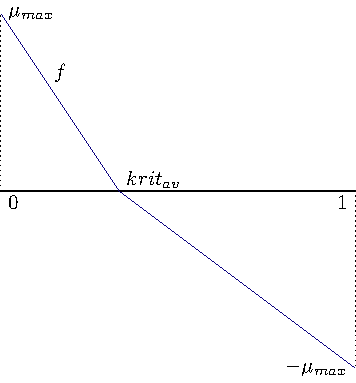
\includegraphics[width = 6cm]{pictures/compiled/erw_prem}
		\caption{Die $\mu$ berechnende Funktion $f$}
		\label{bild:erw_prem}
\end{wrapfigure}
Das erweiterte Premapping durch Schätzen ist in der Lage die Lösungen, welche mit dem Premapping durch Schätzen errechnet wurden, zu verbessern, jedoch geschieht dies nicht regelmäßig. Des Weiteren verursacht der Dijkstra Algorithmus einen nicht zu vernachlässigen Anstieg der Laufzeit. \\
Somit bleibt es offen $f, \mu_{max}$ und $krit_{av}$ so zu wählen, dass eine regelmäßige Verbesserung eintritt. Des Weiteren würde ein Dijkstra Aufruf für jeden Knoten oder eine Beachtung von allen nahezu längsten Wegen eine größere Fülle an Informationen liefern. Da es jedoch nur exponentiell beschränkt viele Wege in $C$ gibt, führt dies zu deutlichen Laufzeiteinbußen. \\

Diese Premapping Methode wird in Kapitel \ref{sec:analyse} aufgrund der nur unregelmäßig auftretenden Verbesserungen nicht behandelt.

\subsection{Preprocessing}
Die Möglichkeiten durch das Matchen sind prinzipiell vielfältig, jedoch bei Gates $p$ mit $|inputs(p)| = fanin_{max}$ auf das beliebige Invertieren der Inputs und des Outputs beschränkt. \\
Um diesem Problem aus dem Weg zu gehen, ist es sinnvoll, vor dem \TM Algorithmus jedes Gate mit mehr als zwei eingehenden Kanten durch einen kleinen Subcircuit, bestehend aus zwei Input Gates, zu ersetzen. Dies ist immer möglich, da jede logische Funktion nur mithilfe von NAND2 und INV Gates realisierbar ist (\cite{Post}) und auf jedem realen Chip standardmäßig ein AND oder NAND sowie ein OR oder NOR in der Library vorhanden sind. INV Gates sind fester Bestandteil jeder realen Library.\\
Dabei werden die Gates nach folgender Routine zerlegt. Eine ausführliche Beschreibung wie Gates mit hohem Eingangsgrad zerlegt werden, befindet sich in \cite{WerberDiss} in Kapitel 2. \\
Der Vorteil des Decompose ist, dass die Möglichkeiten des Technology Mappings deutlich erweitert werden. Jedoch werden für ein AND4 Gate beispielsweise 3 AND2 Gates eingesetzt, was dazu führt, dass sich meist die Kosten des Ausgangscircuits verschlechtern.\\
Eine ausführliche Analyse der Vor- und Nachteile des Decomposens findet sich in Kapitel \ref{sec:analyse}.
	

\subsection{Weitere Optimierungskriterien}
\label{sec:weitere_opt_krit}
Das \TM arbeitet im Chip-Design auf Instanzen realer Chips. Dadurch kommen zu den bereits vorgestellten weitere mögliche Optimierungskriterien hinzu. Es handelt sich hierbei um Kriterien, welche in die Kostenfunktion mit eingebracht werden können und somit während des Technology Mappings optimiert werden. Des Weiteren verursacht der neu implementierte Circuit Kosten, welche im \TM nicht beachtet wurden, für die es jedoch einen übermäßigen Anstieg zu vermeiden gilt. Ein Beispiel hierfür sind die bereits erwähnten zu langen Kanten.\\
Darüber hinaus sind viele Gates teilweise symmetrisch aufgebaut (Bsp.: AND, OR ...) und die Signale der Inputs brauchen unterschiedlich lange zum Output des Gates. Daraus folgt, dass durch Permutierung von Teilmengen der Inputs, Geschwindigkeitsvorteile geschaffen werden können.  
\subsubsection{Pinabhängiges Delay}
\label{subsec:pinabh_delay}
Bis hierhin war das Delay eines Gates als eine nicht negative reelle Zahl definiert. Die meisten Gates besitzen jedoch mehr als nur einen Input. Die Signale der Inputs brauchen nicht alle dieselbe Zeit um zum Output zu gelangen. Logisch werden die Signale der Inputs zwar alle miteinander verrechnet, jedoch geschieht dies physikalisch nicht gleichzeitig und somit müssen nicht alle Signale zur selben Zeit an den Inputs anliegen.\\
Die Möglichkeit eines Signals später an einem Input des Gates ankommen zu können, lässt sich durch einen kleineren Delaywert, spezifisch für diesen Input, realisieren. Denn, wenn das Signal schneller durch das Gate gelangen kann, braucht es auch nicht so früh vorhanden zu sein wie die anderen. \\
Von nun an ist das Delay eines Gates $g$: $d_g \in \mathbb{R}_{\geq 0}^{arity(g)}$. Für das \TM ist dies eine weitere Möglichkeit der Verbesserung, denn viele Gates der Library besitzen mindestens eine Teilmenge von Inputs, welche logisch symmetrisch aufgebaut sind. Diese lassen sich beliebig permutieren. Durch die unterschiedlichen Delay-Eigenschaften der Inputs kann eine solche Permutierung das Delay des Outputs verbessern. Aus diesem Grund ändert sich die AT eines Knotens wie folgt: 
\begin{definition}{AT mit pinabhängigen Delay:}\\
	Sei $C$ ein Circuit und $v \in V(C)$.\\
	Die AT von $v$ mit pinabhängigen Delay ist wie folgt definiert: \[ AT_p(v) :=  \max\limits_{i \in inputs(v)} \{   d_{gate(v),i} + \mathbb{1}_{\{inv_g(i) \}} d_{i} + AT_p(i) + d_{w(k,i)} \}   \}.\]
\end{definition}
Im Folgenden sei mit AT immer das pinabhängige Delay gemeint.

In einem Match ist diese Information bereits abgespeichert, da die Inputs eines Matches mit einer Bijektion an Knoten des Circuits geknüpft werden. Es wird ein  Kandidat für jede mögliche Permutation der Inputs gespeichert, falls dieser nicht dominiert ist.\\
Nach aktuellem Stand gilt $fanin_{max} \leq 4$. Das ist klein genug, um auch bei der Heuristik die max $fanin_{max}$ Permutation bei der Wahl eines Matches in Betracht zu ziehen. 

\subsubsection{Power-Optimierung}
Jedes Gate besitzt neben seinen spezifischen Eigenschaften bezüglich Area und AT noch weitere physikalische Eigenschaften.\\
An einem Transistor liegt immer eine Spannung an. Daraus folgt, dass dieser auch ohne zu schalten Energie (Power) verbraucht. Diese lässt sich einteilen in static Power und dynamic Power. Hierbei bezeichnet static Power den Energieverbrauch unabhängig von der Benutzung des Transistors. Ein Transistor verbraucht jedoch mehr Energie wenn er schaltet. Daraus folgt, dass der Energiebedarf abhängig vom Grad der Nutzung dieses Transistors ist. Dieser variable Energieverbrauch wird auch als dynamic Power bezeichnet.\\
Da ein Gate aus einer logischen Verknüpfung von Transistoren besteht, hat es ebenfalls einen static Power Wert. Da der dynamic Power Wert eines Gates abhängig von der aktuellen Implementierung des Chip ist, ist es schwer, diesen unabhängig von einem Circuit zu errechnen. Aus diesem Grund beschränke ich mich im Folgenden auf die static Power. \\
Die static Power eines Gates korreliert sehr stark mit der physikalischen Größe dieses Bauteils. Aus diesem Grund lassen sich in den oben vorgestellten Algorithmen die Area Daten durch die static Power Werte ersetzen. Der Circuit wird dadurch hinsichtlich Geschwindigkeit und Energiebedarf optimiert. \\
Static Power lässt sich auch zusätzlich zu Area in die Kostenfunktion einbauen. Dies würde bedeuten, dass die Kosten eines Kandidaten $k$ das Tripel $area(k), AT(k), static\_Power(k)$ sind, wobei $static\_Power(k)$ ähnlich wie $area(k)$ errechnet wird. Dies führt jedoch zu einer noch schlechteren Vergleichbarkeit von Kandidaten gleicher und verschiedener Knoten. Aus diesem Grund wird auf die Optimierung aller drei Kriterien zusammen verzichtet. \\
Weitere ausführliche Informationen über Power-Optimierung befinden sich in \cite{Daboul}.\\
In Kapitel \ref{sec:analyse} finden sich weitere Ausführungen über die Auswirkungen von diesem Austausch in der Kostenfunktion.


\section{Resource Sharing}\label{sec:resource_sh}
In diesem Kapitel wird ein weiterer Ansatz für eine Heuristik vorgestellt.\\
Es folgt die allgemeine Definition des Resource Sharing Problems und darauf basierend eine Heuristik, welche sich den Resource Sharing Algorithmus zunutze macht.\\

\subsection{Definition und Lösungsansatz des Resource Sharing Problems}

Eine Instanz des Resource Sharing Problems besteht aus einer endlichen Menge von Kunden $\mathcal{C}$ und einer konvexen Menge $\mathcal{B}_c$ für jeden Kunden $c\in \mathcal{C}$. Diese wird auch Block genannt. Des Weiteren sei $\mathcal{R}$ eine endliche Menge von Ressourcen. Gegeben seien des Weiteren Funktionen $g_c : \mathcal{B}_ c \rightarrow \mathbb{R}^{\mathcal{R}_+}$, welche für jeden Kunden und jedes Element des entsprechenden Blocks einen Ressourcenverbrauch angeben.

Ziel des Resource Sharing ist es, jedem Kunden $c \in \mathcal{C}$ ein Element $b_c \in \mathcal{B}_c$ zuzuordnen, sodass 
\[ \lambda^* := \inf \{ \max\limits_{r \in \mathcal{R}} \sum\limits_{c \in \mathcal{C}}  (g_c(b_c))_r | b_c \in \mathcal{B}_c \forall c \in \mathcal{C} \} \]
approximativ erreicht wird. Mit anderen Worten ist es das Ziel den maximalen Ressourcenverbrauch zu minimieren. 

\subsubsection{Lösungsansatz}
\label{subsec:rs_loesungsansatz}
Der in \cite{Vygen2011} ausführlich beschriebene Lösungsansatz für das Resource Sharing Problem iteriert über die Kundenmenge und errechnet in jeder Iteration mit einem Orakel und Preisen $\omega _r$ für alle Ressourcen $r \in \mathcal{R}$ ein Block Element für jeden Kunden.\\
Das Orakel $f_c : \mathbb{R}^\mathcal{R}_+ \rightarrow \mathcal{B}_c$, auch Blocklöser genannt, wird als gegeben betrachtet und errechnet für gegebene Preise $\omega$ für jedes Element $c \in C$ ein $b_c \in \mathcal{B}_c$ sodass gilt: $ \omega ^T g_c(b_c) \leq \sigma \inf \{ \omega ^T g_c(b) | b \in \mathcal{B}_c \}$ mit einem Approximationsfaktor $\sigma \geq 1$.\\
Nachdem der Blocklöser aufgerufen wurde, wird geprüft ob verknüpfte Ergebnisse der bisherigen Iterationen eine zulässige Lösung der Resource Sharing Instanz liefert. Ist dies nicht der Fall so werden die Preise angepasst und die nächste Iteration mit den neuen Preisen gestartet. Sei $y_r$ die Summe des Ressourcenverbrauchs der Ressource $r$ der vorangegangenen Iterationen. Die Preise werden kontinuierlich durch $\omega _r \rightarrow \omega _r \cdot e^{\gamma \cdot y_r}$ aktualisiert. Hierbei ist $\gamma > 0 $ beliebig, hat jedoch Einfluss auf die Güte der Lösung des Algorithmus.\\

Ist der Algorithmus fertig, liegt das Ergebnis für jeden Kunden in Form einer Konvexkombination von Elementen des zugehörigen Blocks vor. Da jeder Block konvex ist, repräsentiert diese Kombination wieder ein Element des Blocks. \\
Angenommen ein Block ist nicht konvex, muss eine Lösung des Resource Sharing noch zu einem geeigneten Element des zugehörigen Blocks gerundet werden.\\

Das Resource Sharing Problem lässt sich mit einem FPTAS lösen. Ein Beweis hierzu befindet sich in \cite{Vygen2011}.

\subsection{Resource Sharing und \TM}
Der folgende Algorithmus wurde angelehnt an \cite{Daboul2018} entwickelt.\\
Das \TM Problem wird wie folgt durch eine Instanz des Resource Sharing modelliert.\\
Die \TM Instanz bestehe aus einem Circuit $G$ ohne teilweise überflüssige Subcircuits und gegebenen $RAT$'s an den Outputs von $G$. \\
Gesucht sei ein zu $G$ äquivalenter Graph $G*$, dessen Outputsignale vor der entsprechenden $RAT$ ankommen und $Power(G*) \leq B$. Sei $B$ vorerst gegeben. \\
Sei $T_G$ der Timing Graph von $G$. Dieser modelliert alle Delays der Knoten und Kanten von $G$. 
Dieser entsteht aus $G$ indem alle Gate-Knoten $g \in V(G)$ durch $fanin(gate(g)) +1$ Knoten ersetzt werden. Jede der Input-Kanten von $g$ wird durch einen Knoten unterteilt.  Alle Delay-Werte von $G$ lassen sich nun auf $T$ modellieren, 
   \begin{wrapfigure}{r}{2.4cm}
		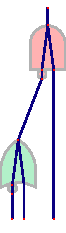
\includegraphics[width = 2.4cm]{pictures/compiled/timing_graph}
		\caption{Beispiel eines Timing Graphen}
		\label{bild:timing_graph}
	\end{wrapfigure}
indem für jede Kante aus $G$ der entsprechenden Kante in $T$ das Delay dieser Kante zugewiesen wird. 
Für jeden Gate-Knoten $g$ aus $G$ werden den entsprechenden Kanten das pinabhängige Delay zugeordnet. Ein Beispiel eines solchen Graphen befindet sich in Abbildung \ref{bild:timing_graph}\\
Sei nun $\mathcal{C} := \{G\} $, $\mathcal{B}_G$ die Menge der nicht dominierten Circuit Kandidaten auf $G$ und $\mathcal{P}_G$ die Menge der inklusionsmaximalen Wege im Timing Graphen von $G$. Die Signale der Outputs eines Graphen kommen genau dann vor der $RAT$ an, wenn  alle $P \in \mathcal{P}$  vor der $RAT$ des zu $P$ gehörenden Outputs ankommen.\\
Somit lässt sich wie folgt festlegen: $\mathcal{R} = \{Power\} \cup \mathcal{P_G}$. \\
Das Orakel in jeder Iteration wird durch eine noch zu beschreibende \TM Heuristik realisiert. \\
Das Ziel dieses Orakels ist, den gewichteten Ressourcenverbrauch
\begin{equation}\label{eq:ressourcen_verbrauch_1}
\omega _{Power} \frac{Power(G)}{B} + \sum\limits_{P \in \mathcal{P}} \omega _P \frac{\sum_{e \in E(P)}Delay_e(G)}{RAT_P}
\end{equation}
 zu minimieren. Hierbei ist $RAT_P$ die $RAT$ des Outputs von $P$.

Durch diese Modellierung des Resource Sharing ergeben sich die folgenden Probleme, welche in den folgenden Unterkapiteln gelöst werden: \\
\begin{itemize}
	\item $|\mathcal{P}|$ ist nur exponentiell beschränkt. Daraus folgt, dass die explizite Speicherung jedes Ressource Preises zu einem nicht polynomiellen Algorithmus führen würde. 
	\item Die \TM Heuristik liefert einen zu $G$ äquivalenten Circuit $G'$. Im Allgemeinen gilt jedoch $\mathcal{P}_G \neq \mathcal{P}_{G'}$. Somit lassen sich keine Ressourcenverbräuche von $G'$ auf den Ressourcen vor dem \TM angeben.
	\item Der Block $\mathcal{B}_G$ ist nicht konvex, wodurch noch eine geeignete Routine zur Rundung anzugeben ist.
\end{itemize}

\subsubsection{Kantenpreise}\label{subsubsec:kantenpreise}
Die Menge $\mathcal{P}_G$ für einen Circuit $G$ ist nur exponentiell beschränkt. Dadurch ist es nicht praktikabel, Preise für jede Pfad Ressource zu speichern. Es ist jedoch möglich, die Preise aller Pfade durch Gewichte auf den Kanten von $T_G$ zu repräsentieren. \\
Seien $(\omega _P)_{P \in \mathcal{P}_G}$ Preise für die Pfad-Ressourcen von $G$. Setze $\omega _e := \sum\limits_{P \in \mathcal{P} : e \in P} \omega _P$.  Die Minimierung von (\ref{eq:ressourcen_verbrauch_1}) durch das Orakel ist nun äquivalent der Minimierung von 
\begin{equation}\label{eq:ressourcen_verbrauch_2}
\omega _{Power} \frac{Power(G)}{B} + \sum\limits_{e \in E(T_G)} \omega_e \frac{Delay_e(G)}{RAT_P}.
\end{equation}
Des Weiteren gilt für $(\omega_e)_{e \in T_G}$ die Flusserhaltung $\sum_{e \in  \delta^- (v)} \omega_e = \sum_{e \in  \delta^+ (v)} \omega_e $.\\

Der Preis eines Pfades lässt sich nun in linearer Zeit errechnen. Ein Beweis dieser Aussage befindet sich in \cite{Haehnle2015}.\\
Neben den Preisen der Pfade lassen sich auch die Summe der Ressourcenverbräuche $y_p$ eines Pfades in Verbräuche der Kanten des Pfades aufteilen. Hierbei gilt: 
\[y_e := \frac{1}{RAT_P} \sum\limits_{k=1}^i \xi^{(k)} \cdot usg^{(k)}(e).\]
Hierbei sind $\xi^{(k)}$ in Iteration $k$ des Algorithmus errechnete Werte in $[0,1]$ und $usg^{(k)}(e)$ entspricht dem der Kante $e$ durch den Algorithmus im folgenden Unterkapitel zugewiesenen Delay.\\
Auf Basis der Verbräuche auf jeder Kante, lassen sich im Resource Sharing Algorithmus die Pfadpreise, repräsentiert durch Kantenpreise,  aktualisieren. \\

Der Algorithmus Edge Weights aktualisiert die Kantenpreise bei gegebenen Ressourcenverbräuchen $(y_e)_{e\in E(T_G)}$ und $\gamma$ in linearer Laufzeit und stammt aus \cite{Daboul2018}. Hierbei gilt für alle Kantenpreise: $\omega_e > 0$. \\

\subsubsection{Ressourcenproblem}
Das \TM Orakel  gibt einen optimierten zu $G$ äquivalenten Circuit $G'$ zurück. Dieser besitzt jedoch neue Pfade und somit eine andere Ressourcenmenge als $G$. 
Pfade aus $G'$ lassen sich jedoch denen aus $G$ zuordnen. Dadurch können die gegebenen Ressourcenverbräuche $(y_e)_{e \in E(T_G)}$ wie folgt aktualisiert werden:
Da jeder Pfad durch ein Match, durch genau eine der eingehenden Kanten des Matches läuft und der Weg eines Pfades durch das Match eindeutig ist, sobald diese Kante bekannt ist, lässt sich der Ressourcenverbrauch des gesamten Weges durch das Match für alle Pfade dieser eingehenden Kante auf eben dieser modellieren. Die eingehenden Kanten eines Matches in $G'$ lassen sich eindeutig Kanten in $G$ zuordnen. \\

Abbildung \ref{bild:RS_new_y} veranschaulicht diese Vorgehensweise. Hierbei entspricht der linke Graph $G$ mit Ressourcenverbräuchen $y_1 ... y_4$ ausgewählter Kanten . Die Ressourcenverbräuche der restlichen Kanten ändern sich durch das dargestellte Match nicht. Der rechte Graph entspricht dem äquivalenten Graph und jeder der Kanten aus $G'$ ist das entsprechende Delay aus $d_1... d_8$ zugeordnet.\\
Jeder der angegebenen Ressourcenverbräuche $y$ wird nun anhand der Summe der Delay-Werte des zu  $y$ korrespondierenden Weges durch das Match aktualisiert. 
Für den Fall, dass mehrere ausgehende eines Knoten zu einer zusammengefasst wurden ( Bsp,: Mux-Match), so werden beide durch die Summe der Delays, dividiert durch die Anzahl der zusammengefassten Kanten, aktualisiert.


\begin{figure}[h]
\begin{center}
 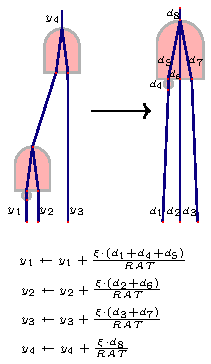
\includegraphics[height = 350pt]{./pictures/compiled/RS_new_y}
 \caption{Beispiel einer Aktualisierung von Ressourcenverbräuchen}
 \label{bild:RS_new_y}
\end{center}
\end{figure}

Diese Routine wird im Folgenden Edge Resources genannt.\\
Wie bereits in Kapitel \ref{subsubsec:klonen} erläutert, ist für die in dieser Arbeit verwendeten \TM Algorithmen das Klonen von Gates nicht erlaubt. Lockert man diese Vorgabe, bleibt es offen zu zeigen, wie Ressourcenverbräuche von neu enstandenen Gates und Kanten in die Aktualisierung der Verbräuche von $G$ eingebracht werden. \\



\begin{comment}
\textcolor{red}{durch kurzen kommentar in letztem Kapitel ersetzen}
Da für die Kantengewichte die Flusserhaltung gilt und die Preise der eingehenden und der ausgehenden Kanten von $G$ \textcolor{red}{oben erklären} gleich bleibt lassen sich durch folgenden Algorithmus entsprechende Kantenpreise auf $G'$ definieren. 

\textcolor{red}{kleinen algo einfügen}

Anhand dieses Algorithmus wird deutlich weshalb $G$ keine teilweise überflüssigen Subcircuits enthalten darf. Mit den teilweise überflüssigen Subcircuits ist es möglich, dass  in $G'$ Inputs ohne ausgehende Kanten existieren. Deren Fluss ließe sich nicht mehr  verteilen. \\

Um das Problem mit der Ressourcenverteilung zu lösen, werden erst mit vorangegangenem Algorithmus Preise für die Kanten von $T_{G'}$ errechnet. Daraufhin werden diese Preise aufgrund der Ressourcenverbräuche in $G'$ aktualisiert. Nach diesem Schritt werden die neuen Kanten Preise von $G'$ wieder in Kantenpreise von $G$ umgewandelt und mit den aktualisierten Preisen wird die nächste Iteration gestartet.\\

Angenommen $G$ besitzt beschränkt viele Multifanoutknoten. In dem Fall ist die Anzahl der Pfade polynomiell beschränkt und die Preise von $G'$ lassen sich in polynomieller Zeit aktualisieren. 
Es bleibt offen zu zeigen, wie Preise von $G'$ ohne diese Einschränkung in polynomieller Laufzeit aktualisiert werde können.\\
\textcolor{red}{oder nur die ye herausfinden!}
\end{comment}
\subsubsection{\TM Orakel}
Das Orakel ist ein \TM Algorithmus mit den folgenden Besonderheiten: \\

Zugrunde gelegt wird die \TM Heuristik aus Kapitel \ref{subsec:heuristik} mit dem Premapping durch Schätzen und erweitert für Circuits mit mehreren Outputs. \\
Damit dieser Algorithmus eine bezüglich der Kantenpreise optimierte Lösung berechnen kann, werden diese wie folgt in dem Algorithmus integriert. \\
Das Delay einer Kante von $G$ wird multipliziert mit dem entsprechenden Preis dieser Kante. Dies gilt ebenfalls für das pinabhängige Delay eines Gates. Das Delay jedes Inputpins eines Gates in $G$ zu seinem Output lässt sich ebenfalls eindeutig einer Kante aus $T_G$ zurordnen. Mit dessen Preis wird auch dieses Delay multipliziert. Des Weiteren werden die Powerwerte der Gates mit $\omega_{Power}$ multipliziert. Da $\omega_e >0$ für jede Kante gilt, führt dies zu positiven Delay-Werten. \\
Durch diese Änderungen minimiert das Orakel heuristisch die Kostenfunktion (\ref{eq:ressourcen_verbrauch_2}).


\subsubsection{Algorithmus}
Im Folgenden wird ein Resource Sharing Algorithmus zur Lösung des Technology Mappings vorgestellt. \\

\LinesNumbered
\begin{algorithm}[H]
\DontPrintSemicolon
\caption{Resource Sharing Algorithmus für das TM}
\SetKwInOut{Task}{Task}
\KwIn{Instanz $G$ des TM-Problems ohne teilweise überflüssige Subcircuits; ein Power-Budget $B$, $\gamma > 0, \, I \in \mathbb{N}$}
\KwOut{Konvexkombination von Kandidaten auf der TM-Instanz}

   $k[\,] \gets \emptyset, \quad \phi[\,] \gets \emptyset, \quad \Xi \gets 0 $\;
  $y_e \gets 0 \quad \forall e \in E(T_G), \quad y_{Power} \gets 0$\;
  \For{$i = 1,...,I$}
     {
        $\omega_{Power} \gets e^{\gamma \cdot y_{Power}}$\;
        $(\omega_e)_{e \in E(T_G)} \gets Edge\_Weights(\gamma, (y_e)_{e \in E(T_G)})$\;
        $k[i] \gets TM\_Oracle(\omega)$\;
        $\xi \gets \min \{ \frac{B}{Power(k[i])}, \frac{RAT_P}{Delay(P)} \forall P \in \mathcal{P}_{k[i}] \}$\;
        \If{$\xi \geq 1$}{\Return $k[i]$}
        $(y_e)_{e \in E(T_G)} \gets Edge\_Resources(k[i], (y_e)_{e \in E(T_G)}, \xi)$\;
        $\phi[i] \gets \xi, \quad \Xi \gets \Xi + \xi$
     }
     \Return $k,\dfrac{\phi}{\Xi}$
\end{algorithm}\ \\

Wenn der Algorithmus nicht in Schritt 9 endet, so nehme man den Kandidaten in $k$ mit dem größten Faktor in ${\phi}/{\Xi}$. Es bleibt offen eine Rounding Methode zu beschreiben, welche jeden berechneten Kandidaten berücksichtigt.

\subsubsection{Abschließende Bemerkungen}
Im bisherigen Verlauf dieses Kapitels wurde $B$ als gegeben vorausgesetzt. Es lässt sich jedoch $B$ durch eine binäre Suche und einem Aufruf des Resource Sharing Algorithmus für jede Iteration der Suche ersetzen. Dies ergibt eine, wenn möglich $RAT$-einhaltende, Lösung mit möglichst kleinem Power-Verbrauch. \\
Des Weiteren lässt sich auch mit einem durch \TM umgebauten Circuit in der nächsten Iteration des Resource Sharing weiterrechnen, jedoch müssen dann die Preise und Ressourcen entsprechend angepasst werden. Dies ist für den gesamten Circuit nicht sinnvoll, da sonst alle Preise evtl. ihre Gültigkeit verlieren. Sehr kritische Subcircuits lassen sich jedoch  mit entsprechenden Veränderungen an Ressourcen und Preisen austauschen. Diese kritischen Bereiche lassen sich auch mithilfe des Preprocessings verändern und in der nächsten Iteration separat bearbeiten. Die Kantenpreise können aufgrund der Flusserhaltung leicht in den neuen Graphen übertragen werden, jedoch ist zu diesem Zeitpunkt noch offen, wie die Summe der Ressourcenverbräuche aufgeteilt auf die Kanten in die neue Umgebung transformiert werden können. Für Graphen mit polynomiell beschränkter Pfadmenge, beispielsweise Graphen mit konstant vielen Multifanoutknoten, lässt sich dies jedoch auch über die Pfadwerte direkt in polynomieller Zeit ändern. \\
Die Definition der Ressourcen und Kunden wurde so allgemein gehalten, dass in einer Iteration des Resource Sharing Algorithmus das \TM sehr einfach durch eine andere die Logik optimierende Routine ausgetauscht werden kann. Abhängig von den aktuellen Preisen und den bisher errechneten Kandidaten ist es möglich, zum Beispiel das \TM Orakel mit  dem  in \cite{Daboul2018} beschriebenen  Gate Sizing Algorithmus zu ersetzen.  Dadurch ist eine deutlich höhere Flexibilität bei der Logik-Optimierung eines Ciruits möglich. \\
Ob der Resource Sharing Algorithmus für das \TM polynomiell implementierbar ist, hängt nur von dem gewählten \TM Algorithmus ab, denn alle anderen Schritte sind wie bereits in Kapitel \ref{subsec:rs_loesungsansatz} beschrieben, polynomiell implementierbar. 

\section{Qualitäts- und Laufzeit-Analyse}
\label{sec:analyse}
In diesem Kapitel werden die vorgestellten Heuristiken bezüglich Laufzeit und Güte analysiert. Vor dieser Analyse ist es jedoch notwendig ein paar Angaben zur Struktur realer Instanzen zu machen, um die Ergebnisse der Algorithmen besser einordnen zu können.\\

Die im Folgenden behandelten Chips liegen mir, aufgrund einer Kooperation zwischen IBM und dem Forschungsinstitut für Diskrete Mathematik in Bonn, vor. Auch die in dieser Arbeit vorgestellten Algorithmen wurden im Rahmen dieses Projektes implementiert. Die Instanzen dieser Chips werden als reale Instanzen bezeichnet.

 \subsection{Struktur realer Instanzen}
\label{subsec:struktur_realer_instanzen} 
Die Instanzen eines Chips sind alle maximal zusammen"-h\"angen\-den, mit \TM vollständig bearbeitbaren, Circuits eines Chips. Da auf einem Chip beispielsweise durch Register gerichtete Kreise entstehen oder Bauteile existieren, welche nicht in der Library vorhanden sind, lässt sich der Logik-Graph eines Chips nicht vollständig mit dem \TM Algorithmus verarbeiten. \\
 Das Chipdesign besteht aus sehr vielen Routinen, welche aus einem Bauplan einen produzierbaren Chip designen. Auf diesem Weg gibt es viele Zwischenstände (Snapshots genannt). Alle getesteten Chips wurden auf dem Stand  des selben Snapshots bearbeitet. Dadurch lassen sich die Verbesserungen von Instanzen durch die Algorithmen miteinander vergleichen auch wenn sie von verschiedenen Chips stammen.\\
 Die folgenden Angaben betrachten alle Instanzen zusammengesetzt zu einem Circuit.
 Insgesamt wurden $1107$ Instanzen getestet. \\

Sei $H_C$ die Menge Multifanouknoten, welche keine Inputs sind, eines Circuits $C$ und $NI_C$ die Menge aller Knoten abz\"uglich der Input-Knoten von $C$. Der durchschnittliche Anteil von $H_C$ an $NI_C$ betr\"agt $30,95\%$. Die Menge der Multifanouknoten, welche ebenfalls Inputs sind, wurde hier nicht beachtet, da diese nur einen m\"oglichen Kandidaten besitzen und somit nicht zu dem Problem des exponentiellen Klassenwachstums beitragen. Diese Werte besitzen bei den gr\"o{\ss}eren Instanzen eine kleine Varianz. Aus diesem Grund werden die Circuits im Folgenden nur anhand ihrer Knotenzahl analysiert.\\
   \begin{wrapfigure}{r}{6cm}
		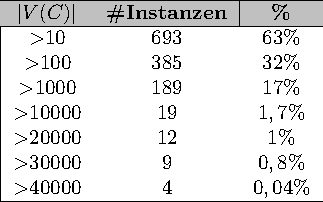
\includegraphics[width = 6cm]{pictures/compiled/instance_sizes_distribution_table}
		\caption{Gr\"o\ss verteilung der getesteten Instanzen}
		\label{bild:sizes_table}
	\end{wrapfigure}
 Der Anteil von Outputs an der Gesamtzahl von Knoten eines Circuits liegt bei $15,26\%$. Von allen Outputs haben $4,13\%$ noch weitere Nachfolger im gleichen Circuit. Outputs mit Nachfolgern werden ebenfalls auf einen Kandidaten beschr\"ankt \textcolor{red}{oben erw\"ahnt ?}, da sie zu den offenen Knoten darauffolgender Knoten gehören. Da diese nur einen solch geringen Anteil an allen Outputs besitzen, werden nur wenige Outputs so fr\"uh festgelegt. Auch hier wurden Outputs, welche auch Inputs sind, aus den gleichen Gr\"unden wie oben, nicht betrachtet.\\
 Die Inputs eines Circuits machen durchschnittlich $16,73\%$ an der Gesamtzahl der Knoten aus. Daraus folgt, dass etwa jeder achte Knoten nur einen Kandidaten tr\"agt. Dies ist bei der Interpretation der folgenden Analysen zu beachten.\\
 Abbildung \ref{bild:sizes_table} zeigt die Verteilung der getesteten Instanzen hinsichtlich der Größe  ihrer Knotenmenge.
 
\textcolor{red}{ Kandidaten menge kann hier noch hin also menge der Kandidaten abh von Knotenmenge bzw anzahl multifanoutknoten  und abh von den oben genannten zusatzfeatures (zb pinabh. delay, Library )  \\  und dass vielleicht die varianz (anhand eines bildes beweisen?) des hoghfanout anteil ziemlich klein ist und somit Knotenmenge und multifanoutmenge ansich ausreichend aussagekräftig sind} 
 
 \subsection{Analyse der Ergebnisse}
 \label{subsec:analyse_der_ergebnisse}

\subsubsection{Tradeoffparameter}
Die Werte von Area, SNS, WS und des Energieverbrauchs eines Circuits liegen selten in derselben Größenordnung. Dies kann zur Folge haben, dass selbst ein vielfacher Verbrauch einer Ressource sich nicht in den Kosten des Circuits-Kandidaten bemerkbar macht. In der Praxis liegen Power, Area oder Arrivaltime häufig um mehrere Zehnerpotenzen auseinander. 

Der Unterschied zwischen dem Verbrauch des Gates mit dem geringsten zu dem Gate mit dem höchsten Ressourcenverbrauch liegt bei maximal Faktor 10.

\begin{wrapfigure}{r}{6cm}
		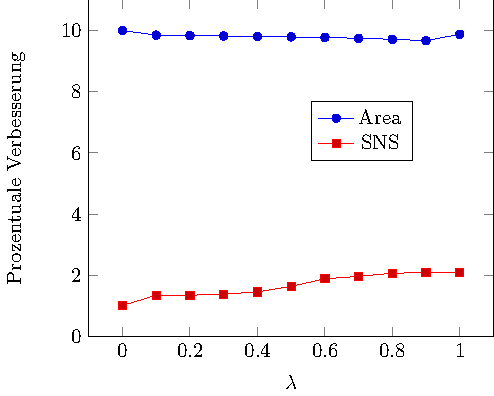
\includegraphics[width = 6cm]{pictures/tex_files/analysis/tradeoff_curve}
		\caption{Einfluss von $\lambda$ auf SNS und Area}
		\label{bild:tradeoff_test}
\end{wrapfigure} 
Der Ressourcenverbrauch eines Gates wird nun durch Dividieren durch den Verbrauch eines sparsamen Gates normalisiert; dann liegen alle Ressourcenverbräuche  in derselben Gr\"o{\ss}enordnung. \\
Im Folgenden wird ausgehend von der \TM Heuristik ohne Preprocessing und mit Premapping durch Sch\"atzen der Einfluss des Tradeoffparameters $\lambda$, abhängig von einer Optimierung nach Area,  auf die Änderung der Kosten untersucht.  Die Kostenfunktion ist hierbei $\lambda SNS(C) + (1-\lambda)Area(C)$.\\
Abbildung \ref{bild:tradeoff_test} veranschaulicht die durchschnittliche prozentuale Verbesserung der Kosten abhängig von $\lambda$.\\


Hier ist nur eine schwache Abh\"angigkeit bez\"uglich des Tradeoffparameters zu erkennen. Dies liegt daran, dass im Schnitt f\"ur jeden dritten Knoten ein Kandidat gesch\"atzt wird. Des Weiteren liegen $SNS$ und $Area$ oft in derselben Gr\"o\ss enordnung, wodurch ein schnellerer Kandidat mit nahezu den gleichen Kosten gesch\"atzt wird wie ein kleinerer und somit unabhängig des $\lambda$, sehr kosten\"ahnliche Kandidaten gew\"ahlt werden; wodurch sich die Kosten des \"aquivalenten Circuits in Abh\"angigkeit des $\lambda$ nur gering ver\"andern.\\
Unabh\"angig von $\lambda$ zeigt die Abbildung \ref{bild:tradeoff_test} jedoch auch ein enormes Verbesserungspotenzial des Circuits in $SNS$ und besonders in $Area$.\\
In folgenden Tests wird aus diesem Grund mit konstantem $\lambda = \frac{1}{2}$ gerechnet.\\

Die Verbessernugen im vorgestellten FPTAS sind sehr stark durch $\lambda$ beeinflusst. Eine ausf\"uhrliche Analyse diese Algorithmus findet sich in \cite{Elbert}.


\subsubsection{Premapping}
Im Folgenden wird das triviale Premapping mit dem Premapping durch Sch\"atzem verglichen. Dies geschieht in Abh\"angigkeit von der Gr\"o{\ss}e der behandelten Instanzen. \\
\begin{figure}[h]
		\centering
		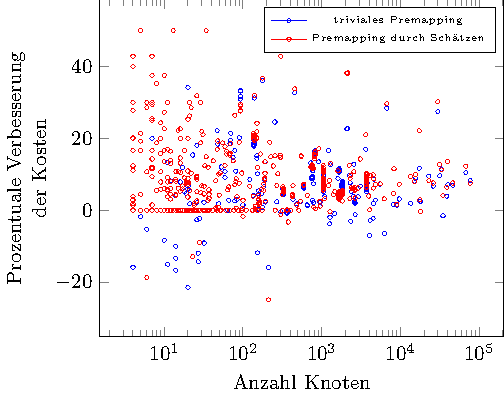
\includegraphics[width = 9cm]{pictures/tex_files/analysis/prem_test}
		\caption{Kostenverbesserung in Abh\"angigkeit der Anzahl von Knoten der Instanzen}
		\label{bild:prem_test}
\end{figure}

Abbildung \ref{bild:prem_test} bildet jeden mit der Heuristik gel\"osten Circuit $C$ bez\"uglich der Anzahl seiner Knoten und der prozentualen Ver\"anderung der Kosten von $C$ ($\lambda \cdot SNS(C) + (1-\lambda) \cdot Area(C)$ ab. Jede Instanz wird einmal mithilfe des trivialen Premappings(blau) und einmal mit dem Premapping durch Sch\"atzen (rot) gel\"ost.\\
Hierbei f\"allt auf, dass sich die Ergebnisse der beiden Premapping Methoden kaum unterscheiden, jedoch wurden mit dem Premapping durch Sch\"atzen deutlich weniger Instanzen gel\"ost deren Kosten nach dem \TM h\"oher sind als vorher. \\

Im Durchschnitt wurden die Kosten der Instanzen durch das triviale Premapping (tP) um $6,74$\% und durch das Premapping durch Sch\"atzen (PdS) um $6,46$\% verbessert. Aufgeteilt auf Area und SNS ergibt sich eine durchschnittliche Verbesserung durch das tP von $8,83$\% Area und $2,75 $\% SNS und mit dem PdS von $10,42$\% Area und $2,16$\% SNS.\\
\begin{wrapfigure}{r}{6cm}
		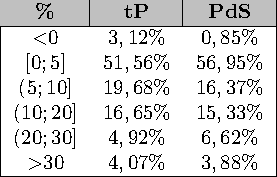
\includegraphics[width = 6cm]{pictures/tex_files/analysis/premapping_table}
		\caption{Verteilung der Kostenverbesserungen}
		\label{bild:premapping_table}
\end{wrapfigure}

Abbildung \ref{bild:premapping_table} gibt einen \"Uberblick \"uber die Verteilung dieser Verbesserungen. Hierbei wird aufgezeigt, wie gro{\ss} der Anteil der Instanzen ist, welche
eine Verbesserung, entsprechend der in der ersten Spalte dargestellten Prozent-Bereiche, erzielt.\\

Aus diesen Gr\"unden ist das Premapping durch Sch\"atzen dem trivialen Premapping vorzuziehen. In den folgenden Tests wird deshalb das Premapping durch Sch\"atzen als Premapping Methode genutzt.

\subsubsection{Preprozessing}
\textcolor{red}{inklusive der graphen größe vergleiche}

\subsubsection{Vergleich von Power und Area}


\subsubsection{Gütevergleich kleiner "optimal " gel instanzen}
\label{subsubsec:guetevgl_kleiner_opt_instanzen}


\subsubsection{Verhalten weiterer Kosten}
\textcolor{red}{die anfallenden kosten die nicht im \TM gemessen werden beobachten und in der future work dran anschließen}

\subsubsection{Zusammenfassung?}
\textcolor{red}{oder am ende nur ein laufzeit güte tradeoff mit eigenem Unterkapitel ?} 
 
 
 \subsection{Laufzeitanalyse}
 \label{subsec:laufzeitanalyse}
Aus der theoretischen Laufzeitschranke aus Kapitel \ref{subsec:heuristik} folgt, dass die Laufzeit maßgeblich von der Menge der Multifanoutknoten abhängt. Andere Faktoren wie das Aufteilen von Gates, die Größe der Library oder die Wahl der Premapping subroutine spielen ebenfalls eine wichtige Rolle. Dies verdeutlicht die Übersicht \textcolor{red}{??}.\\
 Bezüglich der Größe der Library lassen sich die Chips, mit Ausnahme weniger Unterschiede in zwei Gruppen einteilen. Die markierte Teilmenge der Abbildung \textcolor{red}{??} entspricht der Menge der (so genannten) komplexen Gates. Ein Chip lässt sich in der Praxis, abhängig davon, ob er die komplexen Gates grundsätzlich erlaubt, einer der beiden Gruppen zuordnen. Diese Unterscheidung findet sich ebenfalls in Abbildung \textcolor{red}{??}.
 
\subsubsection{Globale Laufzeitanalyse}
\textcolor{red}{welche größenordnungen sind überhaupt lösbar}

\subsubsection{Lokale Laufzeitanalyse}
\textcolor{red}{wie unterscheiden sich die einzelnen Varianten in der Laufzeit? \\ oder lässt sich beides gut in einem bild erkennen ?} \\

\textcolor{red}{hier auch die decompose laufzeit vgl mit rein ?}
 
\subsubsection{Laufzeitverlgeich kleiner "optimal " gel instanzen}


\subsection{Vergleich von Güte und  Laufzeit}
\subsubsection{Kleine Instanzen}

\subsubsection{Allgemein}
\textcolor{red}{wahrscheinlich ist der unterschied bei decompose und ohne am größten den mit der besten premapping methode durchführen}

\section{Fazit und Ausblick}
\label{sec:fazit_und_ausblick}
	

\newpage
\addcontentsline{toc}{section}{\protect\numberline{8}{Literaturverzeichnis}}
\nocite{*}
\renewcommand{\refname}{8 \,\, Literaturverzeichnis}
{ \footnotesize
\bibliography{HeuristikenTM.bib}
\bibliographystyle{alpha}
}
%\clearpage

\end{document}
